% !TeX program = pdflatex
% SOURCE UNIQUE AUTONOME : aucune image ni autre fichier source requis.
% BASCULE : remplacer \proffalse par \proftrue ci-dessous.
% Compilation : pdflatex (deux fois) eleve.tex ou professeur.tex
\documentclass[11pt,a4paper,oneside]{article}
\usepackage[T1]{fontenc}
\usepackage[utf8]{inputenc}
\usepackage[english]{babel}
\usepackage{lmodern,microtype}
\usepackage[a4paper,margin=1.8cm,top=1.8cm,bottom=1.9cm,headheight=15pt]{geometry}
\usepackage{amsmath,amssymb,mathtools,array,tabularx,longtable,multicol}
\usepackage{tikz,pgfplots}
\usetikzlibrary{arrows.meta,calc,patterns,positioning}
\pgfplotsset{compat=1.18}
\usepackage[most]{tcolorbox}
\usepackage{enumitem,fancyhdr,titlesec,needspace,listings,tocloft}
\setlength{\cftsecnumwidth}{3em}
\renewcommand{\cftsecfont}{\normalfont}
\renewcommand{\cftsecpagefont}{\normalfont}
\usepackage[hidelinks,unicode]{hyperref}
\newif\ifprof
\proffalse % <<< REMPLACER PAR \proftrue POUR LA VERSION PROFESSEUR.
\ifdefined\VERSIONPROF\proftrue\fi
\newcommand{\enseignant}{Maths Explorer}
\newcommand{\etablissement}{}
\newcommand{\annee}{2026--2027}
\newcommand{\version}{\ifprof Teacher version\else Student version\fi}
\hypersetup{pdftitle={Mathematics course -- Seconde -- 2026-2027},pdfauthor={Maths Explorer}}
\newcommand{\R}{\mathbb{R}}\newcommand{\N}{\mathbb{N}}\newcommand{\Z}{\mathbb{Z}}\newcommand{\Q}{\mathbb{Q}}\newcommand{\D}{\mathbb{D}}
\newcommand{\vect}[1]{\overrightarrow{#1}}\newcommand{\coord}[2]{\begin{pmatrix}#1\\#2\end{pmatrix}}
\DeclareMathOperator{\Card}{Card}\DeclareMathOperator{\pgcd}{gcd}
\newcounter{sequence}\newcounter{exemple}[sequence]
\renewcommand{\thesection}{\Roman{section}}
\renewcommand{\thesubsection}{\thesection\,--\,\Alph{subsection}}
\newcommand{\titreseq}{}
\renewcommand{\theHsection}{\arabic{sequence}.\arabic{section}}
\pagestyle{fancy}\fancyhf{}
\fancyhead[L]{Seconde}
\fancyhead[R]{\small\itshape Sequence \arabic{sequence}: \titreseq}
\fancyfoot[L]{\small\enseignant}\fancyfoot[C]{\thepage}\fancyfoot[R]{\small\annee}
\renewcommand{\headrulewidth}{0.4pt}\renewcommand{\footrulewidth}{0.4pt}
\titleformat{\section}{\large\bfseries}{\thesection}{1em}{}
\titlespacing*{\section}{0pt}{12pt}{9pt}
\titleformat{\subsection}{\normalsize\bfseries}{\thesubsection}{1em}{}
\setlength{\parindent}{0pt}\setlength{\parskip}{5pt}
\setlist{itemsep=3pt,topsep=5pt,leftmargin=*}
\setlist[enumerate]{label=\arabic*.}
\newcommand{\sequence}[3]{\clearpage\refstepcounter{sequence}\setcounter{section}{0}\renewcommand{\titreseq}{#2}\addcontentsline{toc}{section}{\protect\textbf{Sequence \arabic{sequence}: #1}}\thispagestyle{plain}\begin{tcolorbox}[enhanced,colback=white,colframe=black,boxrule=1pt,arc=2mm,title={Sequence \arabic{sequence}},fonttitle=\bfseries,colbacktitle=black]\centering\Large\bfseries\MakeUppercase{#1}\par\medskip\normalsize\normalfont #3\end{tcolorbox}}
\newcommand{\fiche}[1]{\clearpage\section{#1}}
\newtcolorbox{cours}[1][Property]{enhanced,breakable,colback=white,colframe=black,boxrule=.5pt,arc=2mm,drop shadow=black!35,title={#1},fonttitle=\bfseries,colbacktitle=black,attach boxed title to top left={xshift=0mm,yshift=-1mm},boxed title style={arc=2mm,boxrule=.5pt},top=4mm,bottom=2mm,before skip=10pt,after skip=10pt}
\newtcolorbox{methode}[1][Method]{enhanced,breakable,colback=black!3,colframe=black!60,boxrule=.4pt,arc=0mm,title={#1},colbacktitle=black!15,coltitle=black,fonttitle=\bfseries}
\newcommand{\ex}[2][]{\refstepcounter{exemple}\needspace{4\baselineskip}\par\medskip\textbf{\underline{Example \arabic{sequence}.\arabic{exemple}\if\relax\detokenize{#1}\relax\else: #1\fi}}\par #2\par}
\newcommand{\grille}[1]{\par\smallskip\begin{tikzpicture}\draw[step=.2cm,black!18,very thin] (0,0) grid (16.8,#1);\draw[xstep=.8cm,ystep=.8cm,black!40,thin] (0,0) grid (16.8,#1);\end{tikzpicture}\par}
\newcommand{\reponse}[2][4]{\par\textbf{\underline{Solution:}}\par\ifprof\begin{tcolorbox}[enhanced,breakable,frame hidden,colback=black!3,arc=0mm,borderline west={1pt}{0pt}{black},left=3mm,right=2mm,top=2mm,bottom=2mm]#2\end{tcolorbox}\else\grille{#1}\fi}
\newcommand{\preuve}[2][4]{\par\textbf{Proof to write.}\reponse[#1]{#2}}
\newcommand{\trou}[1]{\ifprof\textbf{#1}\else\makebox[1.1cm]{\dotfill}\fi}
\newcommand{\prof}[1]{\ifprof\begin{methode}[Teacher notes]#1\end{methode}\fi}
\newcommand{\vigilance}[1]{\par\textbf{Watch out.} #1\par}
\newcommand{\rituel}[2]{\begin{methode}[Fluency -- 5 to 10 minutes]#1\end{methode}\ifprof\textit{Answers:} #2\par\fi}
\lstset{language=Python,basicstyle=\small\ttfamily,keywordstyle=\bfseries,commentstyle=\itshape,showstringspaces=false,frame=single,columns=fullflexible,keepspaces=true,breaklines=true,tabsize=4}
\pgfplotsset{coursaxe/.style={axis lines=middle,grid=both,minor tick num=1,width=11cm,height=7cm,xlabel={$x$},ylabel={$y$},tick label style={font=\small},samples=100}}
\begin{document}
\hypersetup{pageanchor=false}
\begin{titlepage}\centering
\rule{\linewidth}{2.5mm}\par\vspace{4mm}
{\fontsize{35}{43}\selectfont\bfseries MATHEMATICS\\COURSE\par}
\vspace{3mm}\rule{\linewidth}{2.5mm}\par\vspace{15mm}
{\fontsize{60}{70}\selectfont\bfseries Seconde\par}
\vspace{10mm}{\Large\version\par}
\vfill{\large \textbf{\enseignant}\par}
\vfill{\Large\annee\par}
\end{titlepage}
\pagestyle{plain}\pagenumbering{roman}\hypersetup{pageanchor=true}
\section*{Organisation of the booklet}
This booklet follows the fifteen stages of the corrected annual plan. The definitions, properties and methods form the course; the examples and proofs are worked in class. The gridded areas are for writing up investigations and solutions. An exercise book can supplement these spaces.
\begin{center}\small\renewcommand{\arraystretch}{1.25}\begin{tabularx}{\linewidth}{c X l}
\textbf{No.}&\textbf{Sequence}&\textbf{Indicative period}\\\hline
1&Arithmetic&2--11 September 2026\\
2&Vectors in the plane&14--30 September\\
3&Straight lines in the plane&1--16 October\\
4&Real numbers and intervals&2--13 November\\
5&Term review and remediation&16--20 November\\
6&Functions: representations and reference functions&23 November--4 December\\
7&Descriptive statistics of one variable&7--18 December\\
8&Algebra, equations and inequalities&4--20 January 2027\\
9&Proportions and percentage change&21--29 January\\
10&Variation and extrema of a function&1--12 February\\
11&Two-way tables of two categorical variables&1--12 March\\
12&Coordinate geometry: synthesis of vectors / lines&15--26 March\\
13&Synthesis problems and reasoning&30 March--9 April\\
14&Probability: conditioning and weighted trees&26 April--24 May\\
15&Consolidation and transition to Première&25 May--11 June\\\hline
\end{tabularx}\end{center}
The dates are progression markers, not a list of teaching days. Public holidays and school holidays are excluded from the sessions, in particular 12 March, 29 March, 6--7 May and 17 May.
\begin{cours}[Annual thread]
Numerical and algebraic calculation, percentages, affine functions, graph reading, reasoning and Python are revisited regularly. There is no initial revision chapter: the fluency exercises are reactivated from the first sequence.
\end{cours}
\prof{The corrected DOCX plan is the reference for order and dates. Reviews 5, 12, 13 and 15 are times for reinvestment. Solutions should only be revealed after an investigation. Exercises explicitly described as fictitious are not real survey data.}
\clearpage\tableofcontents\clearpage\pagenumbering{arabic}\pagestyle{fancy}

\sequence{Arithmetic}{Arithmetic}{2--11 September 2026}
\section{Integers, multiples and divisors}
\begin{cours}[Definitions]
$\N=\{0;1;2;\ldots\}$ is the set of natural numbers. $\Z$ contains the natural numbers and their opposites.
For $a,b\in\Z$, saying that $a$ is a \textbf{multiple of $b$} means that there exists $k\in\Z$ such that $a=bk$. We also say that $b$ divides $a$.
\end{cours}
$18=6\times3$: $18$ is a multiple of $3$ and of $6$. Every integer is a multiple of $1$ and of itself; $0$ is a multiple of every integer. The only multiple of $0$ is $0$.
\ex{List the positive divisors of $18$ and of $24$. Write three multiples of $7$, one of them negative. Is $35$ a multiple of $5$? of $6$? Justify.}
\reponse[4]{Divisors of $18$: $1,2,3,6,9,18$. Divisors of $24$: $1,2,3,4,6,8,12,24$. For example $-7,0,14$ are multiples of $7$. $35=5\times7$ is a multiple of $5$; $35=6\times5+5$ is not a multiple of $6$.}
\begin{cours}[Sum of multiples]
The sum of two multiples of an integer $a$ is a multiple of $a$.
\end{cours}
\preuve[3]{Write $u=ak$ and $v=a\ell$, with $k,\ell\in\Z$. Then $u+v=a(k+\ell)$ and $k+\ell\in\Z$. So $u+v$ is a multiple of $a$. This also holds for $a=0$.}
\rituel{Calculate $\frac23+\frac16$; $3(x+2)-x$; the image of $2$ under $x\mapsto 2x-3$.}{$\frac56$; $2x+6$; $1$.}

\fiche{Parity and prime numbers}
\begin{cours}[Definitions]
An integer $n$ is \textbf{even} if it can be written $2k$, with $k\in\Z$, and \textbf{odd} if it can be written $2k+1$.
A \textbf{prime number} is a natural number greater than or equal to $2$ that has exactly two positive divisors: $1$ and itself.
\end{cours}
The prime numbers less than $100$ are: $2$, $3$, $5$, $7$, $11$, $13$, $17$, $19$, $23$, $29$, $31$, $37$, $41$, $43$, $47$, $53$, $59$, $61$, $67$, $71$, $73$, $79$, $83$, $89$, $97$.
\begin{cours}[Property to prove]
The square of an odd integer is odd.
\end{cours}
\preuve[4]{If $n=2k+1$, then $n^2=(2k+1)^2=4k^2+4k+1=2(2k^2+2k)+1$. Since $2k^2+2k\in\Z$, $n^2$ is odd. The final form justifies the parity; a few numerical trials are not enough to prove the statement.}
\begin{methode}[Testing whether an integer is prime]
For $n\geq2$, it is enough to test the prime divisors less than or equal to $\sqrt n$. Indeed, if $n=ab$ with $1<a\leq b$, then $a\leq\sqrt n$; $a$ has a prime divisor which also divides $n$.
\end{methode}
\ex{Show that $157$ is prime and that $161$ is not.}
\reponse[4]{Since $12^2<157<13^2$, we test $2,3,5,7,11$. None divides $157$: for $7$, $157=7\times22+3$; for $11$, $157=11\times14+3$. So $157$ is prime. On the other hand, $161=7\times23$ is composite.}

\fiche{GCD and irreducible fractions}
\begin{cours}[Definition and convention]
For two integers $a,b$ \textbf{not both zero}, $\pgcd(a,b)$ is the greatest of their common positive divisors. We have $\pgcd(a,b)=\pgcd(|a|,|b|)$ and $\pgcd(a,0)=|a|$ if $a\ne0$. By convention, we set $\pgcd(0,0)=0$; this last case does not come under the definition by the greatest divisor.
\end{cours}
For example, $\pgcd(18,24)=6$, and changing the signs of $18$ or $24$ does not change this result.
\begin{cours}[Prime factorisation -- accepted]
Every natural number greater than or equal to $2$ is a product of prime numbers. This factorisation is unique up to the order of the factors.
\end{cours}
\ex{Factorise $140$, $150$, $630$ and $120$ into prime factors.}
\reponse[3.2]{$140=2^2\times5\times7$; $150=2\times3\times5^2$; $630=2\times3^2\times5\times7$; $120=2^3\times3\times5$. We divide successively by prime numbers and check the final product.}
\begin{methode}[Making a fraction irreducible]
For $b\ne0$, divide the numerator $a$ and the denominator $b$ by $\pgcd(a,b)$. The fraction obtained has a numerator and a denominator that are coprime.
\end{methode}
\ex{Make $\dfrac{140}{630}$, $\dfrac{84}{126}$ and $\dfrac{-120}{150}$ irreducible.}
\reponse[3.2]{The GCDs are $70$, $42$, $30$ respectively. Thus $140/630=2/9$, $84/126=2/3$ and $-120/150=-4/5$. For $140/630$, we can also cancel the factors $2,5,7$ in the factorisations.}

\fiche{Set vocabulary in context}
\begin{cours}[Definitions and notation]
$x\in A$ means that $x$ is an element of $A$; $A\subseteq B$ means that every element of $A$ belongs to $B$. $\varnothing$ is the empty set.
\begin{itemize}
\item $A\cap B$: elements belonging to $A$ \textbf{and} to $B$;
\item $A\cup B$: elements belonging to $A$ \textbf{or} to $B$ (possibly both);
\item in a reference set $E$, $\overline A=E\setminus A$ contains the elements of $E$ that are not in $A$;
\item for a finite set, $\Card(A)$ is its number of elements.
\end{itemize}
\end{cours}
\ex{In $E=\{1;2;3;4;5;6\}$, let $A=\{2;4;6\}$ and $B=\{3;6\}$. Give $A\cap B$, $A\cup B$, $\overline A$ and $\Card(A)$. Are the statements $2\in A$, $\{2\}\subseteq A$ and $A\subseteq B$ true?}
\reponse[3.2]{$A\cap B=\{6\}$, $A\cup B=\{2;3;4;6\}$, $\overline A=\{1;3;5\}$, $\Card(A)=3$. The first two statements are true. The third is false, for example $2\in A$ and $2\notin B$.}
\begin{cours}[Pair and Cartesian product]
A pair $(a,b)$ is ordered: in general $(a,b)\ne(b,a)$. The Cartesian product $A\times B$ is the set of pairs $(a,b)$ with $a\in A$ and $b\in B$. For finite sets, $\Card(A\times B)=\Card(A)\Card(B)$.
\end{cours}
\ex{Write all the elements of $\{1;2\}\times\{3;4;5\}$.}
\reponse[2]{$\{(1,3);(1,4);(1,5);(2,3);(2,4);(2,5)\}$. There are $2\times3=6$ pairs.}

\fiche{Algorithms and putting it to use}
\begin{methode}[Python: integer, Boolean and condition]
\texttt{a \% b} is the remainder of the Euclidean division for integers and $b\ne0$. A test returns a Boolean: \texttt{True} or \texttt{False}. Equality is tested with \texttt{==}; assignment uses \texttt{=}.
\end{methode}
\begin{lstlisting}
def est_multiple(a, b):
    if b == 0:
        return a == 0
    return a % b == 0
\end{lstlisting}
\ex{Predict the results of \texttt{est\_multiple(35, 5)} and \texttt{est\_multiple(35, 6)}, then of \texttt{est\_multiple(0, 7)}, \texttt{est\_multiple(7, 0)} and \texttt{est\_multiple(0, 0)}. Explain the role of the condition.}
\reponse[3]{The results are \texttt{True}, \texttt{False}, \texttt{True}, \texttt{False}, \texttt{True}. The case $b=0$ avoids calculating a remainder modulo zero, which is impossible, and applies the definition: only $0$ is a multiple of $0$.}
\ex[Problem]{We have $84$ notebooks and $126$ pencils. We want to make as many identical packs as possible, using all the material. How many packs can we make? What does each contain?}
\reponse[4]{The number of packs divides $84$ and $126$. Its maximum is therefore $\pgcd(84,126)=42$. Each pack contains $84/42=2$ notebooks and $126/42=3$ pencils. The check $42\times2=84$, $42\times3=126$ confirms that all the material is used.}
\prof{Diagnostic: have students state ``divides'' and ``is a multiple of''. Help: start by testing 2, 3, 6 packs. Extension: prove that $n(n+1)$ is even by distinguishing the two parities of $n$.}

\sequence{Vectors in the plane}{Vectors in the plane}{14--30 September 2026}
\section{Translation and vectors}
\begin{cours}[Definition]
The translation that transforms $A$ into $B$ associates with every point $M$ the unique point $M'$ such that $ABM'M$ is a parallelogram, possibly flat. It is called the translation by the vector $\vect{AB}$.
A nonzero vector has a direction, a sense and a norm. $\|\vect{AB}\|=AB$. The vector $\vect{AA}$ is the zero vector, written $\vec0$; it has neither direction nor sense.
\end{cours}
\begin{center}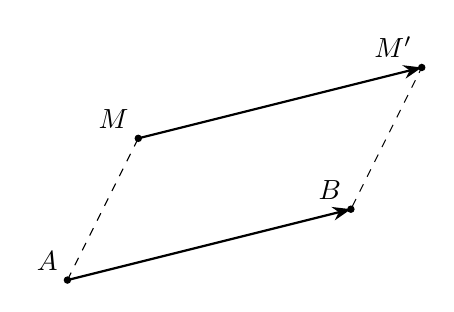
\begin{tikzpicture}[>=Stealth,scale=.9]
\coordinate(A) at (0,0);\coordinate(B) at (4,1);\coordinate(M) at (1,2);\coordinate(N) at (5,3);
\draw[dashed](A)--(M)--(N)--(B);\draw[->,thick](A)--(B);\draw[->,thick](M)--(N);
\foreach \p/\n in {A/A,B/B,M/M,N/M'}\fill(\p)circle(1.5pt) node[above left]{$\n$};
\end{tikzpicture}\end{center}
\begin{cours}[Equal and opposite vectors]
$\vect{AB}=\vect{CD}$ when the translation by the vector $\vect{AB}$ transforms $C$ into $D$. Two nonzero vectors are equal if and only if they have the same direction, the same sense and the same norm.
The opposite vector of $\vect{AB}$ is $\vect{BA}$: $\vect{BA}=-\vect{AB}$.
\end{cours}
\ex{Draw a segment $[AB]$ and place a point $C$ outside $(AB)$. Construct $D$ such that $\vect{AB}=\vect{CD}$. Name the parallelogram obtained. Construct $E$ such that $\vect{CE}=-\vect{AB}$.}
\reponse[4]{$D$ is constructed by carrying over from $C$ the direction, sense and length of $\vect{AB}$. The parallelogram is $ABDC$, in that order. $E$ is the reflection of $D$ in the point $C$, because $\vect{CE}=-\vect{CD}$.}

\fiche{Sum, difference and Chasles's relation}
\begin{cours}[Sum of vectors]
The sum $\vec u+\vec v$ corresponds to carrying out the translations by the vectors $\vec u$ and $\vec v$ one after the other. For all points $A,B,C$:
\[\boxed{\vect{AB}+\vect{BC}=\vect{AC}}\qquad\text{(Chasles's relation).}\]
We have $\vec u-\vec v=\vec u+(-\vec v)$ and $\vect{AB}+\vect{BA}=\vec0$.
\end{cours}
\begin{center}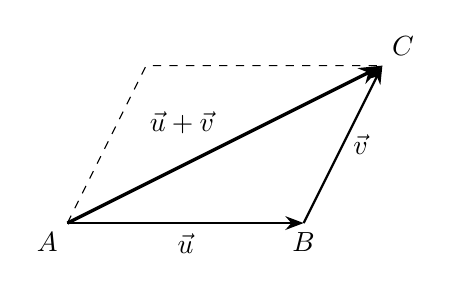
\begin{tikzpicture}[>=Stealth,scale=1.0]
\draw[->,thick](0,0)--(3,0)node[midway,below]{$\vec u$};
\draw[->,thick](3,0)--(4,2)node[midway,right]{$\vec v$};
\draw[->,very thick](0,0)--(4,2)node[midway,above left]{$\vec u+\vec v$};
\draw[dashed](0,0)--(1,2)--(4,2);
\node[below left]at(0,0){$A$};\node[below]at(3,0){$B$};\node[above right]at(4,2){$C$};
\end{tikzpicture}\end{center}
\begin{cours}[Parallelogram rule]
$ABDC$ is a parallelogram if and only if $\vect{AD}=\vect{AB}+\vect{AC}$.
\end{cours}
\ex{Simplify: $\vect{AB}+\vect{BC}$; $\vect{AB}+\vect{CA}$; $\vect{AB}+\vect{BC}+\vect{CD}$; $\vect{AB}-\vect{AC}$.}
\reponse[3.2]{$\vect{AC}$; $\vect{CA}+\vect{AB}=\vect{CB}$; $\vect{AD}$; $\vect{AB}+\vect{CA}=\vect{CB}$. The commutativity of addition allows us to reorder the vectors.}
\ex{In a parallelogram $ABCD$, justify that $\vect{AB}+\vect{AD}=\vect{AC}$.}
\reponse[2.4]{In $ABCD$, $\vect{AD}=\vect{BC}$. So $\vect{AB}+\vect{AD}=\vect{AB}+\vect{BC}=\vect{AC}$.}

\fiche{Product of a vector by a real number}
\begin{cours}[Definition and calculation rules]
For $k\in\R$, $k\vec u=\vec0$ if $k=0$ or $\vec u=\vec0$. Otherwise, $k\vec u$ has the same direction as $\vec u$, the same sense if $k>0$, the opposite sense if $k<0$, and its norm is $|k|\|\vec u\|$.
\[(k+\ell)\vec u=k\vec u+\ell\vec u,\quad k(\vec u+\vec v)=k\vec u+k\vec v,\quad k(\ell\vec u)=(k\ell)\vec u.\]
\end{cours}
\ex{For a vector $\vec u$ of norm $4$ cm, represent $2\vec u$, $-\vec u$ and $\frac12\vec u$ from the same origin. State their norms.}
\reponse[3.2]{The norms are $8$ cm, $4$ cm, $2$ cm. The vectors $2\vec u$ and $\frac12\vec u$ have the sense of $\vec u$; $-\vec u$ has the opposite sense.}
\begin{cours}[Characterisations of the midpoint]
$I$ is the midpoint of $[AB]$ if and only if $\vect{AI}=\vect{IB}$, or equivalently $\vect{AI}=\frac12\vect{AB}$, or $\vect{IA}+\vect{IB}=\vec0$.
\end{cours}
\ex{In a triangle $ABC$, $I$ is the midpoint of $[AB]$ and $J$ that of $[AC]$. Show that $\vect{IJ}=\frac12\vect{BC}$.}
\reponse[4.4]{By Chasles, $\vect{IJ}=\vect{IA}+\vect{AJ}=-\frac12\vect{AB}+\frac12\vect{AC}=\frac12(\vect{BA}+\vect{AC})=\frac12\vect{BC}$. We recover the parallelism of the lines $(IJ)$ and $(BC)$ when the triangle is not flat.}
\rituel{Simplify $3\vec u-5\vec u$; calculate $(-3)^2$; solve $2x+1=7$.}{$-2\vec u$; $9$; $x=3$.}

\fiche{Frames, bases and coordinates}
\begin{cours}[Definitions]
Two non-collinear vectors $\vec i,\vec j$ form a basis of the plane. Every vector $\vec u$ can be written uniquely as $\vec u=x\vec i+y\vec j$; its coordinates are $(x;y)$ or $\coord{x}{y}$.
A frame $(O;\vec i,\vec j)$ associates with the point $M$ the coordinates of $\vect{OM}$. It is \textbf{orthonormal} if the basis vectors are perpendicular and of norm $1$.
\end{cours}
\begin{center}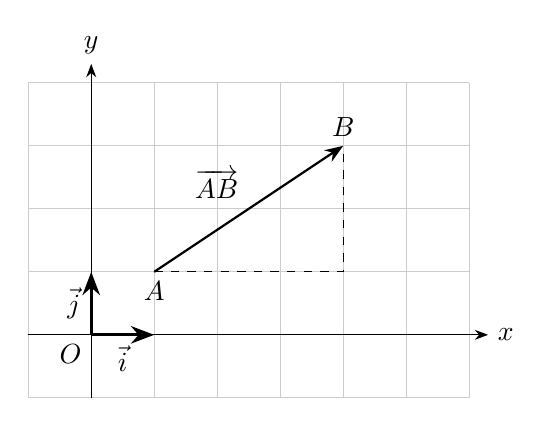
\begin{tikzpicture}[>=Stealth,scale=.8]
\draw[step=1,black!20](-1,-1)grid(6,4);\draw[->](-1,0)--(6.3,0)node[right]{$x$};\draw[->](0,-1)--(0,4.3)node[above]{$y$};
\draw[->,very thick](0,0)--(1,0)node[midway,below]{$\vec i$};\draw[->,very thick](0,0)--(0,1)node[midway,left]{$\vec j$};
\draw[->,thick](1,1)--(4,3)node[midway,above left]{$\vect{AB}$};\draw[dashed](1,1)--(4,1)--(4,3);
\node[below]at(1,1){$A$};\node[above]at(4,3){$B$};\node[below left]at(0,0){$O$};
\end{tikzpicture}\end{center}
Here $\vect{AB}=3\vec i+2\vec j$: we move three units to the right and two upwards.
\begin{cours}[Calculations with coordinates]
If $A(x_A;y_A)$, $B(x_B;y_B)$, $\vec u(x;y)$ and $\vec v(x';y')$:
\[\vect{AB}=\coord{x_B-x_A}{y_B-y_A},\quad \vec u+\vec v=\coord{x+x'}{y+y'},\quad k\vec u=\coord{kx}{ky}.\]
Two vectors are equal if and only if their respective coordinates are equal.
\end{cours}
\ex{For $\vec u(3;2)$ and $\vec v(-1;4)$, calculate $\vec u+\vec v$ and $2\vec u-\vec v$. Write $\vec w(5;-3)$ in the basis $(\vec i,\vec j)$.}
\reponse[2.4]{$\vec u+\vec v=(2;6)$; $2\vec u-\vec v=(7;0)$; $\vec w=5\vec i-3\vec j$.}

\fiche{Norm, distance and midpoint}
\begin{cours}[Properties]
In an \textbf{orthonormal} frame, for $\vec u(x;y)$ and two points $A,B$:
\[\|\vec u\|=\sqrt{x^2+y^2},\qquad AB=\sqrt{(x_B-x_A)^2+(y_B-y_A)^2}.\]
In any frame, the midpoint of $[AB]$ is $I\left(\frac{x_A+x_B}{2};\frac{y_A+y_B}{2}\right)$.
\end{cours}
\preuve[3]{The distance formula follows from Pythagoras's theorem applied to the horizontal and vertical displacements. For the midpoint, $\vect{AI}=\frac12\vect{AB}$ gives $x_I-x_A=\frac{x_B-x_A}{2}$ and $y_I-y_A=\frac{y_B-y_A}{2}$; we isolate $x_I,y_I$.}
\ex{In an orthonormal frame, $A(3;0)$, $B(5;3)$, $C(4;0)$ and $D(6;4)$.
\begin{enumerate}
\item Calculate $\vect{AB}$, $\vect{CD}$, then $3\vect{AB}-5\vect{CD}$.
\item Determine $U$ such that $\vect{BU}=2\vect{AB}-\vect{CD}$.
\item Determine $E$ such that $ABCE$ is a parallelogram, then its centre $I$.
\item Calculate $AB$ and $CD$.
\end{enumerate}}
\reponse[6]{1. $\vect{AB}=(2;3)$ and $\vect{CD}=(2;4)$, so $3\vect{AB}-5\vect{CD}=(-4;-11)$.\\
2. $\vect{BU}=(2;2)$, so $U=B+(2;2)=(7;5)$.\\
3. $E=A+C-B=(2;-3)$. The centre is the midpoint of $[AC]$: $I(7/2;0)$. The midpoint of $[BE]$ gives the same result.\\
4. $AB=\sqrt{13}$ and $CD=\sqrt{20}=2\sqrt5$.}

\fiche{Collinearity and determinant}
\begin{cours}[Definition]
Two nonzero vectors are collinear if they have the same direction. The zero vector is collinear with every vector. If $\vec v\ne\vec0$, $\vec u$ and $\vec v$ are collinear if and only if there exists a real number $k$ such that $\vec u=k\vec v$.
\end{cours}
\vigilance{In the last characterisation, the condition $\vec v\ne\vec0$ is necessary: a nonzero vector cannot be a multiple of the zero vector.}
\begin{cours}[Determinant and collinearity criterion]
For $\vec u(x;y)$, $\vec v(x';y')$, $\det(\vec u,\vec v)=xy'-yx'$.
\[\vec u,\vec v\text{ collinear}\quad\Longleftrightarrow\quad\det(\vec u,\vec v)=0.\]
\end{cours}
\preuve[4.2]{If $\vec u=k\vec v$, then $xy'-yx'=kx'y'-ky'x'=0$. The case where a vector is zero is immediate.
Conversely, suppose $\vec v\ne\vec0$ and $xy'-yx'=0$. If $x'\ne0$, let $k=x/x'$. The equality gives $y=ky'$, so $\vec u=k\vec v$. If $x'=0$, then $y'\ne0$, hence $x=0$; with $k=y/y'$, we again obtain $\vec u=k\vec v$.}
\ex{Study the collinearity of: (a) $\vec u(3;2)$ and $\vec v(-6;-5)$; (b) $\vec w(4;1)$ and $\vec t(3;3/4)$. If $\vect{AB}=2\vect{CD}$ and $\vect{BD}=-5\vect{CD}$, relate $\vect{AB}$ and $\vect{BD}$.}
\reponse[3.2]{(a) $\det(\vec u,\vec v)=-15+12=-3\ne0$: not collinear. (b) $\vec t=\frac34\vec w$: collinear; the determinant is $4\times\frac34-3=0$. Finally $\vect{AB}=-\frac25\vect{BD}$, including if the vectors are zero.}

\fiche{Alignment and parallelism}
\begin{cours}[Applications]
For $A\ne B$ and $C\ne D$, the lines $(AB)$ and $(CD)$ are parallel (possibly coincident) if and only if $\det(\vect{AB},\vect{CD})=0$.
The points $A,B,C$ are collinear if and only if $\det(\vect{AB},\vect{AC})=0$.
\end{cours}
\ex{Show that $(AB)$ and $(CD)$ are parallel with $A(2;-4)$, $B(10;-2)$, $C(-16;-4)$ and $D(12;3)$.}
\reponse[3.2]{$\vect{AB}=(8;2)$ and $\vect{CD}=(28;7)$. Their determinant is $8\times7-2\times28=0$. The points of each pair are distinct: both lines exist and are parallel.}
\ex{Show that $E(0;1/2)$, $F(2;1)$ and $G(6;2)$ are collinear.}
\reponse[3.2]{$\vect{EF}=(2;1/2)$ and $\vect{EG}=(6;3/2)=3\vect{EF}$. The determinant is $2\times3/2-(1/2)\times6=0$; so the points are collinear.}
\ex{With $A(-1;1)$, $B(3;2)$, $C(-2;-3)$, $D(6;-1)$, $E(5;0)$, show that $(AB)\parallel(CD)$ and that $E,B,D$ are collinear.}
\reponse[3.2]{$\vect{AB}=(4;1)$ and $\vect{CD}=(8;2)=2\vect{AB}$. Then $\vect{EB}=(-2;2)$ and $\vect{ED}=(1;-1)=-\frac12\vect{EB}$. Both results follow.}

\sequence{Straight lines in the plane}{Straight lines in the plane}{1--16 October 2026}
\section{Direction vector and Cartesian equation}
\begin{cours}[Definition]
A direction vector of a line is a \textbf{nonzero} vector having the direction of that line. If $A\ne B$, $\vect{AB}$ directs $(AB)$.
Every line has an equation $ax+by+c=0$ with $(a,b)\ne(0,0)$. A direction vector is $\coord{-b}{a}$.
\end{cours}
\ex{For $A(-2;4)$ and $B(6;2)$, calculate $\vect{AB}$ then check that $\vec u(4;-1)$ directs $(AB)$.}
\reponse[2.4]{$\vect{AB}=(8;-2)=2\vec u$. The vector $\vec u$ is nonzero and collinear with $\vect{AB}$; it therefore directs $(AB)$.}
\begin{cours}[Establishing an equation with the determinant]
The line through $A(x_A;y_A)$ with direction vector $\vec u(\alpha;\beta)\ne\vec0$ has equation
\[\beta(x-x_A)-\alpha(y-y_A)=0.\]
\end{cours}
\preuve[4]{A point $M(x;y)$ belongs to the line if and only if $\vect{AM}$ is collinear with $\vec u$, including for $M=A$. Now
\[\det(\vect{AM},\vec u)=(x-x_A)\beta-(y-y_A)\alpha.\]
Setting the determinant to zero gives the stated equation. Expanding, $a=\beta$, $b=-\alpha$ and $c=-\beta x_A+\alpha y_A$; since $\vec u\ne\vec0$, $(a,b)\ne(0,0)$.}
\vigilance{The zero vector directs no line. The sign of the determinant depends on the order of the vectors, but whether it vanishes does not.}

\fiche{Determining the equation of a line}
\begin{methode}
From a point and a direction vector: choose $a,b$ then replace $x,y$ by the coordinates of the point to find $c$. From two distinct points: first calculate a direction vector.
\end{methode}
\ex{Determine a Cartesian equation of the line through $A(2;-1)$ with direction vector $\vec u(3;2)$.}
\reponse[4]{$a=2$, $b=-3$ will do. The line therefore has an equation $2x-3y+c=0$. Since $A$ belongs to it, $4+3+c=0$, so $c=-7$. An equation is $2x-3y-7=0$. Check: $2\times2-3\times(-1)-7=0$ and $(3;2)$ is indeed a direction vector.}
\ex{Determine a Cartesian equation of $(AB)$ for $A(3;3)$ and $B(2;-2)$.}
\reponse[4]{$\vect{AB}=(-1;-5)$ directs the line. We can choose $(a,b)=(5,-1)$. With $A$, $15-3+c=0$, so $c=-12$. Thus $5x-y-12=0$. For $B$, $10+2-12=0$, which confirms the result.}
\ex{Does the point $P(1;2)$ belong to $d:2x-3y+4=0$? Does the point $Q(2;1)$ belong to it?}
\reponse[2.4]{For $P$, $2-6+4=0$: yes. For $Q$, $4-3+4=5\ne0$: no.}

\fiche{Slope-intercept equation, slope and affine function}
\begin{cours}[Definitions]
A non-vertical line has a unique slope-intercept equation $y=mx+p$. $m$ is the slope, $p$ the y-intercept. It represents the affine function $x\mapsto mx+p$; $(1;m)$ is a direction vector.
A vertical line has an equation $x=k$; it is not the graph of a function of $x$. A horizontal line has an equation $y=k$.
\end{cours}
\begin{cours}[Calculating a slope]
If $x_A\ne x_B$, the slope of $(AB)$ is $m=\dfrac{y_B-y_A}{x_B-x_A}$. To find $p$, we then use $y_A=mx_A+p$.
\end{cours}
\ex{Determine the slope-intercept equation of $2x+3y-1=0$, then draw $d:y=-2x+3$.}
\reponse[2.4]{$3y=-2x+1$, so $y=-\frac23x+\frac13$. For $d$, plot $(0;3)$ and $(1;1)$, then draw the line; a move of $1$ along the x-axis corresponds to $-2$ on the y-axis.}
\begin{center}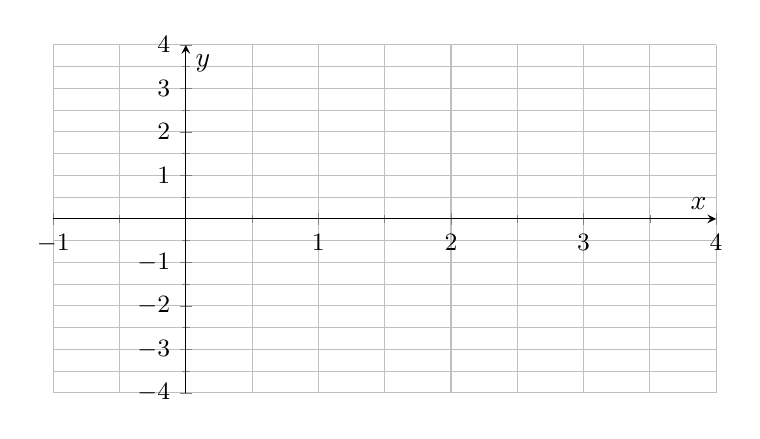
\begin{tikzpicture}\begin{axis}[coursaxe,xmin=-1,xmax=4,ymin=-4,ymax=4,width=10cm,height=6cm,xtick={-1,...,4},ytick={-4,...,4}]
\ifprof\addplot[thick,domain=-.5:3.5]{-2*x+3};\addplot[only marks]coordinates{(0,3)(1,1)};\fi
\end{axis}\end{tikzpicture}\end{center}
\ex{Find the affine function $f$ such that $f(0)=3$ and $f(-1)=5$, then the affine function $g$ whose graph passes through $C(-1;2)$ and $E(5;-2)$.}
\reponse[2.4]{$f(x)=-2x+3$, since $m=(3-5)/(0+1)=-2$. For $g$, $m=(-2-2)/(5+1)=-2/3$ and $p=2-2/3=4/3$, so $g(x)=-\frac23x+\frac43$.}

\fiche{Relative positions of two lines}
\begin{cours}[Properties]
Two lines are either intersecting, strictly parallel or coincident. For $y=mx+p$ and $y=m'x+p'$:
\begin{itemize}\item if $m\ne m'$, they intersect;\item if $m=m'$ and $p\ne p'$, they are strictly parallel;\item if $m=m'$ and $p=p'$, they coincide.\end{itemize}
For Cartesian equations, we compare the directions with the determinant. If the directions are collinear, we then test the membership of a point to distinguish coincident lines from strictly parallel ones.
\end{cours}
\ex{Determine an equation of $d$ through $A(2;3)$ and parallel to $d':x-3y-3=0$.}
\reponse[3.2]{$d'$ has direction vector $(3;1)$. We look for $d:x-3y+c=0$. Since $A\in d$, $2-9+c=0$, so $c=7$. Thus $d:x-3y+7=0$. The two lines are strictly parallel, because the constants differ for the same coefficients of $x,y$.}
\ex{Study the relative positions:
\begin{enumerate}\item $2x-y+1=0$ and $4x-2y+2=0$;\item $x=2$ and $x=-1$;\item $y=2x-3$ and $y=-x+3$.\end{enumerate}}
\reponse[4]{1. The second equation is twice the first: coincident lines. 2. Two distinct vertical lines: strictly parallel. 3. The slopes $2$ and $-1$ differ: intersecting. Their intersection satisfies $2x-3=-x+3$, so $x=2$ and $y=1$.}

\fiche{Intersection: solving by substitution}
\begin{cours}[Definition]
Solving a system of two equations in $x,y$ means finding all the pairs $(x;y)$ satisfying both equations simultaneously. For two equations of lines: an intersection gives one solution pair; strictly parallel lines give no solution; coincident lines give infinitely many solutions.
\end{cours}
\begin{methode}[Substitution]
Isolate one unknown in one equation, substitute its expression into the other, solve, then find the second unknown. Check the pair in both original equations.
\end{methode}
\ex{Solve $\begin{cases}-2x+y+3=0,\\3x-5y-2=0.\end{cases}$}
\reponse[4]{The first equation gives $y=2x-3$. Substituting into the second: $3x-5(2x-3)-2=0$, that is $-7x+13=0$. Thus $x=13/7$ then $y=5/7$. The solution set is $S=\{(13/7;5/7)\}$. The substitutions give $(-26+5+21)/7=0$ and $(39-25-14)/7=0$.}
\ex{Solve by substitution:
\[\text{(a) }\begin{cases}-2x+y+3=0\\x-4y+5=0\end{cases}\qquad
\text{(b) }\begin{cases}2x+3y-10=0\\4x+5y-16=0.\end{cases}\]}
\reponse[4]{(a) $y=2x-3$ then $x-4(2x-3)+5=0$, so $x=17/7$, $y=13/7$.\\(b) $x=(10-3y)/2$; $2(10-3y)+5y-16=0$, so $y=4$, then $x=-1$.}

\fiche{Linear combination and Python}
\begin{methode}[Linear combination]
Multiply the equations by nonzero numbers to obtain opposite coefficients for one unknown; add them to eliminate that unknown. Keep one equation of the system to calculate the other unknown.
\end{methode}
\ex{Solve $\begin{cases}2x+3y+1=0\\3x-4y-2=0.\end{cases}$ Then redo the two systems of the previous example by linear combination.}
\reponse[4.8]{Multiplying the first equation by $3$ and the second by $-2$ gives $6x+9y+3=0$ and $-6x+8y+4=0$. The sum gives $17y+7=0$, so $y=-7/17$. Then $2x-21/17+1=0$, so $x=2/17$.
For (a), add four times the first equation to the second: $-7x+17=0$, so $(x;y)=(17/7;13/7)$. For (b), subtract twice the first from the second: $-y+4=0$, so $(x;y)=(-1;4)$.}
\begin{lstlisting}
def determinant(u, v):
    return u[0]*v[1] - u[1]*v[0]

def alignes(A, B, C):
    AB = (B[0]-A[0], B[1]-A[1])
    AC = (C[0]-A[0], C[1]-A[1])
    return determinant(AB, AC) == 0
\end{lstlisting}
\ex{Predict \texttt{alignes((0,0), (2,1), (6,3))} then \texttt{alignes((0,0), (2,1), (6,4))}.}
\reponse[2]{\texttt{True}, then \texttt{False}: the determinants are $0$ and $2$. The exact test is suitable here for integer coordinates; floating-point approximations require taking numerical errors into account.}

\sequence{Real numbers and intervals}{Real numbers and intervals}{2--13 November 2026}
\section{Sets of numbers}
\begin{cours}[Definitions]
\begin{itemize}
\item $\N$: natural numbers; $\Z$: integers.
\item $\D$: decimal numbers, of the form $a/10^n$ with $a\in\Z$, $n\in\N$.
\item $\Q$: rational numbers, of the form $a/b$ with $a,b\in\Z$, $b\ne0$.
\item $\R$: real numbers, represented by the abscissae of the points of a graduated line. A real number that is not rational is \textbf{irrational}.
\end{itemize}
\[\N\subsetneq\Z\subsetneq\D\subsetneq\Q\subsetneq\R.\]
\end{cours}
\begin{center}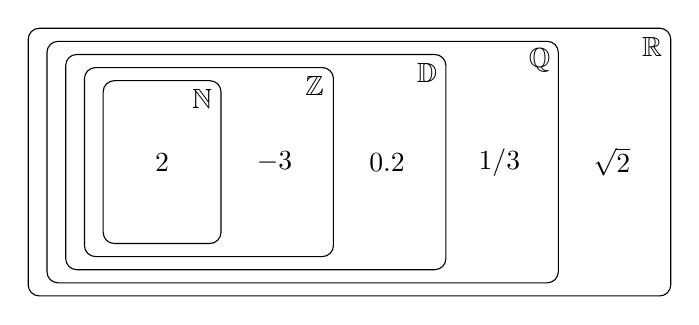
\begin{tikzpicture}[scale=.68]
\foreach \x/\w/\label in {0/12/\R,.35/9.9/\Q,.7/7.8/\D,1.05/5.7/\Z,1.4/3.6/\N}{\draw[rounded corners](\x,\x*.7)rectangle(\w,5-\x*.7);\node at(\w-.35,4.65-\x*.7){$\label$};}
\node at(2.5,2.5){$2$};\node at(4.6,2.5){$-3$};\node at(6.7,2.5){$0.2$};\node at(8.8,2.5){$1/3$};\node at(10.9,2.5){$\sqrt2$};
\end{tikzpicture}\end{center}
\ex{Give the smallest of the five sets containing each of the numbers: $-95$; $7.29$; $5/3$; $\sqrt{25}$; $\sqrt2$; $\pi$; $0.0002$.}
\reponse[3.2]{$-95\in\Z$; $7.29\in\D$; $5/3\in\Q$; $\sqrt{25}=5\in\N$; $\sqrt2,\pi\in\R\setminus\Q$; $0.0002=2/10^4\in\D$. The irrationality of $\pi$ is accepted here.}

\fiche{Two proofs by contradiction}
\begin{methode}[Proof by contradiction]
To prove a statement, assume its negation, deduce a contradiction, then conclude that the statement is true.
\end{methode}
\begin{cours}[Property]
$\dfrac13$ is not a decimal number.
\end{cours}
\preuve[5]{Suppose $1/3=a/10^n$ with $a\in\Z$, $n\in\N$. Then $10^n=3a$ would be a multiple of $3$. Yet $10\equiv1$ modulo $3$, so $10^n$ leaves remainder $1$ on division by $3$ (the divisibility rule for $3$ can also be used). Contradiction. Hence $1/3\notin\D$.}
\begin{cours}[Property]
$\sqrt2$ is irrational.
\end{cours}
\preuve[6]{Suppose $\sqrt2=p/q$ with $p,q\in\N$, $q\ne0$, and $p/q$ in lowest terms. Then $p^2=2q^2$, so $p^2$ is even. If $p$ were odd, its square would be odd: so $p$ is even. Write $p=2k$. We get $4k^2=2q^2$, then $q^2=2k^2$; so $q$ is even in turn. Thus $2$ divides $p$ and $q$, contradicting irreducibility. Hence $\sqrt2\notin\Q$.}
\prof{Have students identify separately the starting hypothesis, the implication used by contraposition on parity, and the final contradiction. Do not present a calculator's decimal expansion as a proof of irrationality.}

\fiche{Intervals of the real line}
\begin{cours}[Notation]
For two real numbers $a<b$, intervals describe the real numbers lying between two endpoints, with or without the endpoints. A closed bracket includes the endpoint, an open bracket excludes it. The symbols $-\infty,+\infty$ are not real numbers and are always paired with an open bracket.
\end{cours}
\begin{center}\renewcommand{\arraystretch}{1.8}\begin{tabular}{c|c|l}
\textbf{Condition}&\textbf{Interval}&\textbf{Description}\\\hline
$a\leq x\leq b$&$[a;b]$&both endpoints included\\
$a<x\leq b$&$]a;b]$&$a$ excluded, $b$ included\\
$a\leq x<b$&$[a;b[$&$a$ included, $b$ excluded\\
$a<x<b$&$]a;b[$&both endpoints excluded\\
$x\geq a$&$[a;+\infty[$&greater than or equal to $a$\\
$x>a$&$]a;+\infty[$&strictly greater than $a$\\
$x\leq b$&$]-\infty;b]$&less than or equal to $b$\\
$x<b$&$]-\infty;b[$&strictly less than $b$
\end{tabular}\end{center}
\[\R=]-\infty;+\infty[,\quad \R^*=]-\infty;0[\,\cup\,]0;+\infty[.\]
\vigilance{The strictly negative real numbers form $]-\infty;0[$: $0$ is excluded. $[a;a]=\{a\}$; $]a;a[=\varnothing$.}
\ex{Write as an interval then represent: $2\leq x\leq5$; $x>4$; $-6<x\leq2$; $x<0$.}
\reponse[4]{$[2;5]$; $]4;+\infty[$; $]-6;2]$; $]-\infty;0[$. On the number line, mark the endpoints, then show each one as included or excluded.}

\fiche{Intersection and union of intervals}
\begin{cours}[Definition]
$\,I\cap J$ corresponds to the condition ``belonging to $I$ \textbf{and} to $J$''; $I\cup J$ corresponds to ``belonging to $I$ \textbf{or} to $J$''. A union of intervals is not always an interval.
\end{cours}
\ex{With $I=[0;12]$ and $J=[3;20]$, determine $I\cap J$ and $I\cup J$.}
\reponse[2.4]{$I\cap J=[3;12]$ and $I\cup J=[0;20]$.}
\ex{Complete, justifying with representations on a number line.}
\begin{center}\renewcommand{\arraystretch}{2}\begin{tabular}{c c|c c}
$I$&$J$&$I\cap J$&$I\cup J$\\\hline
$]-4;3]$&$[1;5]$&\trou{$[1;3]$}&\trou{$]-4;5]$}\\
$]-\infty;2]$&$[-4;+\infty[$&\trou{$[-4;2]$}&\trou{$\R$}\\
$]-\infty;7]$&$[7;+\infty[$&\trou{$\{7\}$}&\trou{$\R$}\\
$]-\infty;5]$&$[-3;+\infty[$&\trou{$[-3;5]$}&\trou{$\R$}\\
$]-2;0[$&$]0;3]$&\trou{$\varnothing$}&\trou{$]-2;0[\cup]0;3]$}
\end{tabular}\end{center}
\reponse[4]{For each intersection, keep the points common to both representations; for each union, keep all the points of at least one. In the last row, $0$ belongs to neither interval: the union cannot be replaced by $]-2;3]$.}
\rituel{Simplify $\vect{AB}+\vect{BC}$; solve $3x-6=0$; calculate $10^{-2}$.}{$\vect{AC}$; $x=2$; $0.01$.}

\fiche{Absolute value and distance}
\begin{cours}[Definition and properties]
$|x|$ is the distance from the real number $x$ to $0$; $|x|\geq0$ and
\[|x|=\begin{cases}x&\text{if }x\geq0,\\-x&\text{if }x<0.\end{cases}\]
The distance between $a$ and $b$ is $|b-a|$. For $a\in\R$ and $r\geq0$:
\[|x-a|\leq r\iff x\in[a-r;a+r],\qquad |x-a|<r\iff x\in]a-r;a+r[.\]
\end{cours}
\ex{Calculate $|3.2|$, $|-1.6|$, $|\sqrt3-2|$, then the distances between $2$ and $5$, $2$ and $-5$, $-2$ and $-5$.}
\reponse[2.4]{$3.2$; $1.6$; $2-\sqrt3$ since $\sqrt3<2$. The distances are $3$, $7$ and $3$.}
\ex{Solve: $|x-7/3|=14$; $|x-2|\leq3$; $|x+3|<5$.}
\reponse[4.8]{For the first equation, $x-7/3=14$ or $x-7/3=-14$, so $S=\{-35/3;49/3\}$. Then $|x-2|\leq3\iff x\in[-1;5]$. Finally $|x+3|=|x-(-3)|<5\iff x\in]-8;2[$.}
\ex{Write $x\in[4;10]$ as an inequality with an absolute value.}
\reponse[2]{The centre is $(4+10)/2=7$ and the radius $(10-4)/2=3$: $|x-7|\leq3$.}

\fiche{Bounds and approximations}
\begin{cours}[Vocabulary]
To bound $x$ is to give $a\leq x\leq b$; the width is $b-a$. An approximation from below is less than or equal to $x$; an approximation from above is greater than or equal to it. Rounding chooses the nearest value at the required precision.
Significant figures are counted from the first nonzero digit; the displayed precision must suit the context.
\end{cours}
\ex{Bound $\sqrt2$ between two consecutive hundredths. Give its rounding to the nearest hundredth. Round $0.004567$ to three significant figures, then $12345$ to three significant figures in scientific notation.}
\reponse[3.2]{$1.41^2=1.9881<2<2.0164=1.42^2$, so $1.41<\sqrt2<1.42$ (width $0.01$). The rounding to the nearest hundredth is $1.41$. The other roundings are $0.00457$ and $1.23\times10^4$.}
\begin{lstlisting}
def encadre_racine2(p):
    # p entier naturel ; calculs entiers exacts
    q = 10**p
    k = 0
    while (k+1)**2 <= 2*q*q:
        k = k+1
    return k/q, (k+1)/q
\end{lstlisting}
\ex{Explain why this function bounds $\sqrt2$. What does it return for $p=2$? Why does it terminate?}
\reponse[3.2]{The loop looks for the largest integer $k$ such that $k^2\leq2q^2$. On exit, $k^2\leq2q^2<(k+1)^2$, so $k/q\leq\sqrt2<(k+1)/q$. For $p=2$, it returns $(1.41;1.42)$. Since $(2q)^2>2q^2$, the counter eventually reaches a value that makes the test false. The final divisions are floating-point approximations; the square tests are exact.}

\sequence{Term review and remediation}{Term review}{16--20 November 2026}
\section{Individual review}
\begin{methode}[Instructions]
Work without the course notes for 25 minutes, then check with the methods in the booklet. For each question, note: solved alone, solved with help, or to redo. Justify the answers.
\end{methode}
\ex[Review of sequences 1 to 4]{\begin{enumerate}
\item Reduce $90/126$ to lowest terms. Prove that the sum of two odd integers is even.
\item With $A(-1;2)$ and $B(3;-2)$, calculate $\vect{AB}$, $AB$ and the midpoint of $[AB]$ in an orthonormal frame.
\item Determine an equation of $(AB)$; does $C(5;-4)$ belong to this line?
\item Calculate $[-2;4]\cap]1;7]$ and $[-2;4]\cup]1;7]$.
\item Solve $|x-1|\leq4$ and explain why $1/3\notin\D$.
\end{enumerate}}
\reponse[9]{1. $\pgcd(90,126)=18$, so $90/126=5/7$. If $u=2k+1$ and $v=2\ell+1$, then $u+v=2(k+\ell+1)$ is even.\\2. $\vect{AB}=(4;-4)$; $AB=4\sqrt2$; midpoint $I(1;0)$.\\3. $y=-x+1$. For $C$, $-4=-5+1$: it belongs to $(AB)$.\\4. Intersection $]1;4]$; union $[-2;7]$.\\5. $x\in[-3;5]$. Writing $1/3=a/10^n$ would require $10^n$ to be divisible by $3$, which is impossible.}
\prof{Possible marking out of 20: 4 points per question. Assess calculation skill, choice of method and quality of justification separately.}
\fiche{Correcting an error and revisiting a method}
\ex[Analysis of student work]{Correct: (a) ``$\vect{AB}=(x_A-x_B;y_A-y_B)$''; (b) ``The zero vector directs every line''; (c) ``$|x-2|\leq3$ gives $x\in[2;3]$''; (d) ``$1/3\approx0.333$, so $1/3$ is decimal''.}
\reponse[5]{(a) Subtract the origin from the endpoint: $(x_B-x_A;y_B-y_A)$. (b) A direction vector must be nonzero. (c) The distance to $2$ is at most $3$: $x\in[-1;5]$. (d) $0.333$ differs from $1/3$: $3\times0.333=0.999\ne1$. A decimal approximation does not determine the nature of the approximated number.}
\ex[Remediation track]{\begin{enumerate}
\item Reduce $72/108$, then $\frac34-\frac16$.
\item With $P(1;1)$ and $Q(5;3)$, determine the midpoint, a direction vector and an equation of $(PQ)$.
\item Determine $]-\infty;3]\cap[-1;+\infty[$, then solve $|x+2|<1$.
\end{enumerate}}
\reponse[5]{1. $2/3$; $7/12$. 2. Midpoint $(3;2)$, direction vector $(2;1)$, equation $x-2y+1=0$. 3. Intersection $[-1;3]$; solution of the inequality $]-3;-1[$.}
\fiche{Applying and self-assessing}
\ex[Synthesis problem]{Two displacements are represented by $\vec u(6;4)$ and $\vec v(9;6)$.
\begin{enumerate}\item Show that they are collinear and find the coefficient relating $\vec v$ to $\vec u$.
\item The starting point is $A(-2;1)$. Determine the endpoints $B$ and $C$ associated with the displacements $\vec u$ and $\vec v$.
\item Find an equation of the line through these three points.
\item A point $M(x;y)$ of this line must satisfy $|x-4|\leq3$. Give the interval of possible abscissae.
\end{enumerate}}
\reponse[7]{1. $\vec v=\frac32\vec u$. 2. $B(4;5)$ and $C(7;7)$. 3. A direction vector is $(3;2)$; the equation is $2x-3y+7=0$, satisfied by the three points. 4. $|x-4|\leq3\iff x\in[1;7]$.}
\begin{cours}[My review]
My priority: \dotfill\par The mistake to avoid: \dotfill\par The method to reuse: \dotfill\par An exercise to redo without help: \dotfill
\end{cours}
\prof{Validate the remediation with a similar exercise done without help after a delay. Orally, ask for a sentence linking the calculation to the geometric conclusion.}

\sequence{Functions: representations and reference functions}{Functions: representations}{23 November--4 December 2026}
\section{Function, image and preimage}
\begin{cours}[Definition]
A real-valued function associates to each real number $x$ of its domain $D_f$ a unique real number $f(x)$, called the image of $x$. A preimage of $y$ is a real number $x\in D_f$ such that $f(x)=y$. We write $f:x\mapsto f(x)$. A number may have no preimage, one, or several.
\end{cours}
\ex{Let $g(x)=x^2-4x+32$ on $\R$. Calculate $g(-5)$. Let $h(x)=3x+5$; determine the preimage of $6$ under $h$.}
\reponse[3.2]{$g(-5)=25+20+32=77$: $77$ is the image of $-5$, and $-5$ is a preimage of $77$. For $h$, $3x+5=6\iff x=1/3$. The only preimage is $1/3$.}
\ex{For the square function, calculate the images of $-3$ and $3$, then the preimages of $9$, $0$ and $-1$.}
\reponse[3.2]{$f(-3)=f(3)=9$. The preimages of $9$ are $-3,3$; $0$ has a single preimage, $0$; $-1$ has none in $\R$.}
\begin{lstlisting}
def g(x):
    return x*x - 4*x + 32
\end{lstlisting}
\ex{Distinguish \texttt{g(-5)} from \texttt{x = -5}.}
\reponse[2]{The first calls the function and returns $77$. The second assigns $-5$ to the variable \texttt{x}, without calculating the image under $g$.}
\fiche{Domain of definition}
\begin{cours}[Conditions for existence]
$D_f$ contains the values for which the process defining $f$ makes sense. A denominator must be nonzero; a number under a square root must be positive or zero. Also respect any domain imposed by the statement or the context.
\end{cours}
\ex{Determine the domains of definition:
\[f(x)=3x^2-5x+2,\quad g(x)=\frac{2x+1}{x-4},\quad h(x)=\frac{x}{x^2-9},\quad k(x)=\sqrt{2x-6}.\]}
\reponse[5]{$D_f=\R$. $D_g=]-\infty;4[\cup]4;+\infty[$ since $x-4\ne0$. $D_h=]-\infty;-3[\cup]-3;3[\cup]3;+\infty[$ since $x^2-9\ne0$. $D_k=[3;+\infty[$ since $2x-6\geq0$.}
\vigilance{The square root of a negative number does not exist in $\R$; it is not ``a negative square root'' that is excluded.}
\ex[Modelling]{A rectangle of perimeter $20$ m has width $x$ m. Express its area and state the domain if both dimensions must be strictly positive.}
\reponse[5]{The length is $10-x$, so $A(x)=x(10-x)$ in m$^2$. $x>0$ and $10-x>0$ give $D_A=]0;10[$. If degenerate rectangles were allowed, we could take $[0;10]$.}
\fiche{Table of values and representative curve}
\begin{cours}[Definition]
$\mathcal C_f$ is the set of points $(x;f(x))$, with $x\in D_f$. Thus $M(a;b)\in\mathcal C_f\iff a\in D_f$ and $b=f(a)$.
\end{cours}
\ex{On $[-1;4]$, $f(x)=x^2-2x-1$. Complete the table, then draw the curve over the whole interval.}
\begin{center}\renewcommand{\arraystretch}{1.6}\begin{tabular}{c|rrrrrrrr}
$x$&$-1$&$-0.5$&$0$&$1$&$1.5$&$2$&$3$&$4$\\\hline
$f(x)$&\trou{$2$}&\trou{$0.25$}&$-1$&$-2$&\trou{$-1.75$}&$-1$&\trou{$2$}&\trou{$7$}
\end{tabular}\end{center}
\begin{center}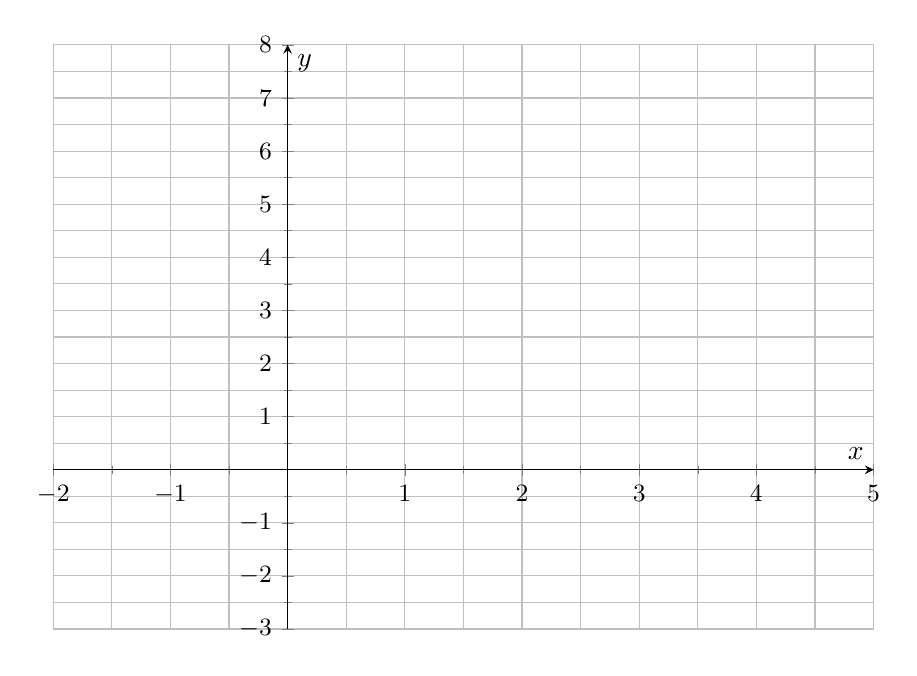
\begin{tikzpicture}\begin{axis}[coursaxe,xmin=-2,xmax=5,ymin=-3,ymax=8,width=12cm,height=9cm,xtick={-2,...,5},ytick={-3,...,8}]
\ifprof\addplot[thick,domain=-1:4]{x*x-2*x-1};\addplot[only marks]coordinates{(-1,2)(-.5,.25)(0,-1)(1,-2)(1.5,-1.75)(2,-1)(3,2)(4,7)};\fi
\end{axis}\end{tikzpicture}\end{center}
\reponse[2]{Images: $2$; $0.25$; $-1$; $-2$; $-1.75$; $-1$; $2$; $7$. Plot the points then draw the parabola. Segments joining only these points would give just an approximation.}
\fiche{Graphical solving of equations and inequalities}
\begin{cours}[Method]
The solutions of $f(x)=k$ are the abscissae of the intersections of $\mathcal C_f$ with $y=k$. For $f(x)\leq k$, read the abscissae where the curve is below this line, intersections included; with $<$, the intersections are excluded.
\end{cours}
\ex{The curve represents $f(x)=1+\frac14(x+3)(x+1)(x-2)$ on $[-4;3]$. Solve graphically $f(x)=1$, $f(x)\leq1$ and $f(x)>1$.}
\begin{center}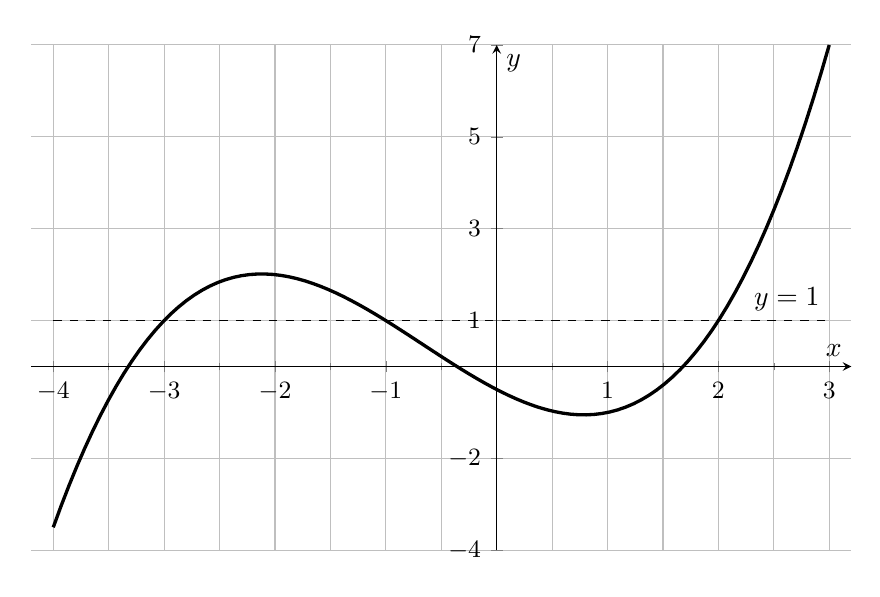
\begin{tikzpicture}\begin{axis}[coursaxe,xmin=-4.2,xmax=3.2,ymin=-4,ymax=7,xtick={-4,...,3},ytick={-4,-2,0,1,3,5,7},width=12cm,height=8cm]
\addplot[very thick,domain=-4:3]{1+(x+3)*(x+1)*(x-2)/4};\addplot[dashed,domain=-4:3]{1};\node[anchor=south east]at(axis cs:3,1){$y=1$};
\end{axis}\end{tikzpicture}\end{center}
\reponse[4]{$f(x)=1$: $-3,-1,2$. $f(x)\leq1$: $[-4;-3]\cup[-1;2]$. $f(x)>1$: $]-3;-1[\cup]2;3]$. The endpoints $-4,3$ come from the domain. The factorisation checks the intersections exactly; the algebraic study of the sign will be consolidated in sequence 8.}
\prof{Graph rebuilt to replace an ambiguous reading in the original booklet. Distinguish graphical conjecture from exact validation.}
\fiche{Comparing two functions; reading a sign}
\begin{cours}[Method]
$f(x)=g(x)$ is read at the intersections of the curves. For $f(x)<g(x)$, $\mathcal C_f$ is strictly below $\mathcal C_g$ at the same abscissa. The sign of $f(x)$ is read relative to the x-axis.
\end{cours}
\ex{On $[-3;3]$, $f(x)=x^2$ and $g(x)=x+2$. Solve $f=g$, $f<g$, $f\geq g$ and determine the sign of $g$.}
\begin{center}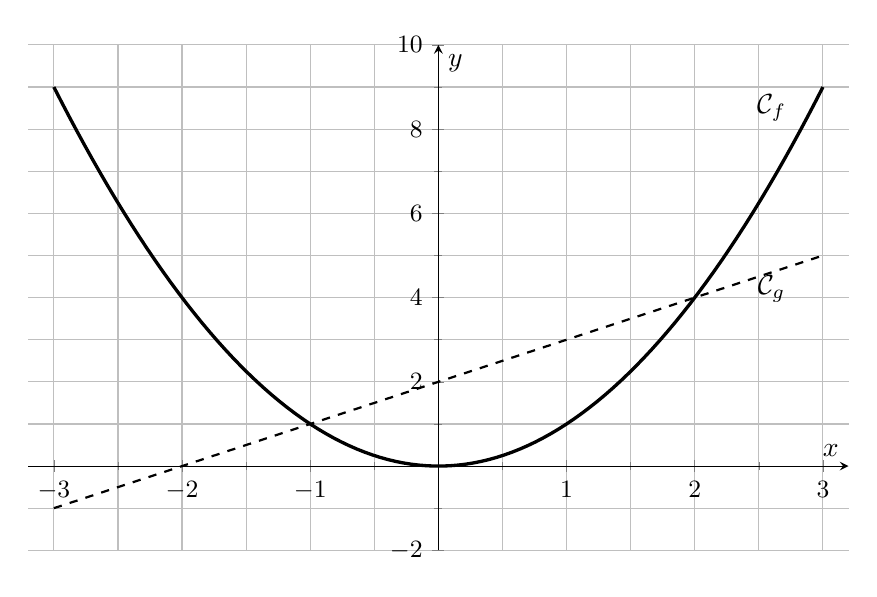
\begin{tikzpicture}\begin{axis}[coursaxe,xmin=-3.2,xmax=3.2,ymin=-2,ymax=10,width=12cm,height=8cm,xtick={-3,...,3},ytick={-2,0,2,4,6,8,10}]
\addplot[very thick,domain=-3:3]{x*x};\addplot[thick,dashed,domain=-3:3]{x+2};\node at(axis cs:2.6,8.5){$\mathcal C_f$};\node at(axis cs:2.6,4.2){$\mathcal C_g$};
\end{axis}\end{tikzpicture}\end{center}
\reponse[4]{$f=g$ for $x=-1,2$; $f<g$ on $]-1;2[$; $f\geq g$ on $[-3;-1]\cup[2;3]$. $g$ is strictly negative on $[-3;-2[$, zero at $-2$, strictly positive on $]-2;3]$. Sign and variations are different pieces of information.}
\fiche{Affine functions and absolute value}
\begin{cours}[Definitions]
An affine function is $f(x)=mx+p$ on $\R$. It is linear if $p=0$, constant if $m=0$. For $m\ne0$, it vanishes at $-p/m$; its sign is that of $m$ to the right of this number.
The function $x\mapsto|x|$ is defined on $\R$, positive or zero, and vanishes only at $0$.
\end{cours}
\ex{Classify (several answers possible) as affine, linear, constant: $5x+2$; $5x$; $7+2x-7$; $6$; $6(4x-2)$; $6x+5-6x$.}
\reponse[2.4]{All are affine. $5x$ and $2x$ are linear; $6$ and $5$ are constant; $24x-12$ is neither linear nor constant.}
\begin{center}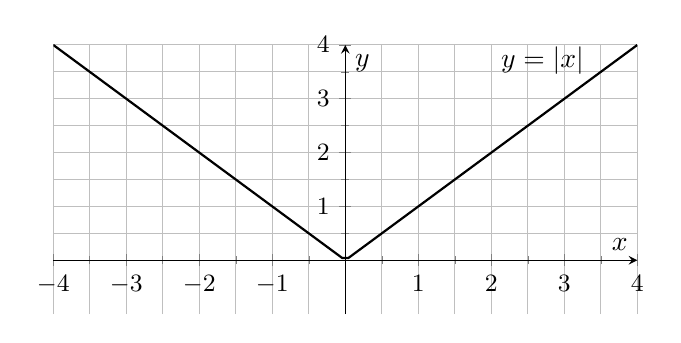
\begin{tikzpicture}\begin{axis}[coursaxe,xmin=-4,xmax=4,ymin=-1,ymax=4,width=9cm,height=5cm,xtick={-4,...,4},ytick={0,...,4}]
\addplot[thick,domain=-4:4]{abs(x)};\node at(axis cs:2.7,3.7){$y=|x|$};\end{axis}\end{tikzpicture}\end{center}
\begin{cours}[Equations and inequalities]
If $k<0$, $|x|=k$ and $|x|\leq k$ have no solution, and $|x|\geq k$ is true on $\R$. If $k=0$, the first two give $x=0$, the third is true on $\R$. For $k>0$:
\[|x|=k\iff x\in\{-k;k\},\quad |x|\leq k\iff x\in[-k;k],\]
\[|x|\geq k\iff x\in]-\infty;-k]\cup[k;+\infty[.\]
\end{cours}
\ex{Solve $|x|=5$, $|x|=-3$, $|x|\leq3$, $|x|\geq4$.}
\reponse[1.6]{$\{-5;5\}$; $\varnothing$; $[-3;3]$; $]-\infty;-4]\cup[4;+\infty[$.}
\fiche{Square and inverse functions}
\begin{cours}[Definitions and sign]
$x\mapsto x^2$ is defined on $\R$; its curve is a parabola. $x^2\geq0$, with equality only at $0$.
$x\mapsto1/x$ is defined on $\R^*$; its curve is a hyperbola. $1/x$ has the sign of $x$ and never vanishes.
\end{cours}
\begin{center}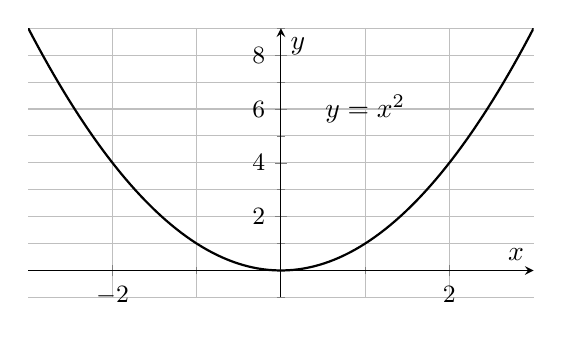
\begin{tikzpicture}\begin{axis}[coursaxe,xmin=-3,xmax=3,ymin=-1,ymax=9,width=8cm,height=5cm,xtick={-2,0,2}]
\addplot[thick,domain=-3:3]{x*x};\node at(axis cs:1,6){$y=x^2$};\end{axis}\end{tikzpicture}
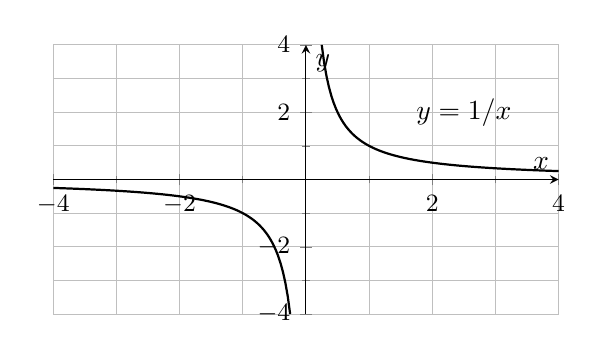
\begin{tikzpicture}\begin{axis}[coursaxe,xmin=-4,xmax=4,ymin=-4,ymax=4,width=8cm,height=5cm,xtick={-4,-2,0,2,4}]
\addplot[thick,domain=-4:-.25]{1/x};\addplot[thick,domain=.25:4]{1/x};\node at(axis cs:2.5,2){$y=1/x$};\end{axis}\end{tikzpicture}\end{center}
\begin{cours}[Equations and inequalities with $x^2$]
If $k<0$, $x^2=k$ and $x^2\leq k$ have no solution; $x^2\geq k$ is true on $\R$. If $k=0$, the first two give $x=0$, the third is true on $\R$. For $k>0$:
\[x^2=k\iff x\in\{-\sqrt k;\sqrt k\},\quad x^2\leq k\iff x\in[-\sqrt k;\sqrt k],\]
\[x^2\geq k\iff x\in]-\infty;-\sqrt k]\cup[\sqrt k;+\infty[.\]
\end{cours}
\ex{Solve $x^2=4$, $x^2=-1$, $x^2\geq4$, $x^2\geq-1$, $1/x=4$, $1/x=0$.}
\reponse[3.2]{$\{-2;2\}$; $\varnothing$; $]-\infty;-2]\cup[2;+\infty[$; $\R$; $\{1/4\}$; $\varnothing$. More generally, $1/x=k$ has the unique solution $1/k$ if $k\ne0$, none if $k=0$.}
\fiche{Inequalities with the inverse function}
\begin{methode}
Respect $x\ne0$ and read both branches of the hyperbola. Do not multiply an inequality by $x$ without knowing its sign.
\end{methode}
\begin{center}\small\renewcommand{\arraystretch}{2.5}\begin{tabular}{c|c|c|c}
&$k<0$&$k=0$&$k>0$\\\hline
$1/x\leq k$&$[1/k;0[$&$]-\infty;0[$&$]-\infty;0[\cup[1/k;+\infty[$\\
$1/x\geq k$&$]-\infty;1/k]\cup]0;+\infty[$&$]0;+\infty[$&$]0;1/k]$
\end{tabular}\end{center}
\ex{Solve $1/x\geq2$, $1/x\leq-1$, $1/x<1/2$ and $1/x>-2$.}
\reponse[5]{$]0;1/2]$; $[-1;0[$; $]-\infty;0[\cup]2;+\infty[$; $]-\infty;-1/2[\cup]0;+\infty[$. A strict inequality excludes the intersection with $y=k$; $0$ is always forbidden.}
\ex{A student writes: ``$1/x\leq2\iff1\leq2x$, so $x\geq1/2$''. What is missing?}
\reponse[4]{They implicitly assumed $x>0$. For $x<0$, $1/x<0<2$: these values also work. The correct set is $]-\infty;0[\cup[1/2;+\infty[$. The number $-1$ refutes their equivalence.}
\fiche{Using square root and cube}
\begin{cours}[Definitions]
$x\mapsto\sqrt x$ is defined on $[0;+\infty[$ and takes values that are positive or zero. For $k\geq0$, $\sqrt x=k\iff x=k^2$; for $k<0$, no solution.
$x\mapsto x^3$ is defined on $\R$. Every real number $k$ has a unique preimage, written $\sqrt[3]{k}$.
\end{cours}
\begin{center}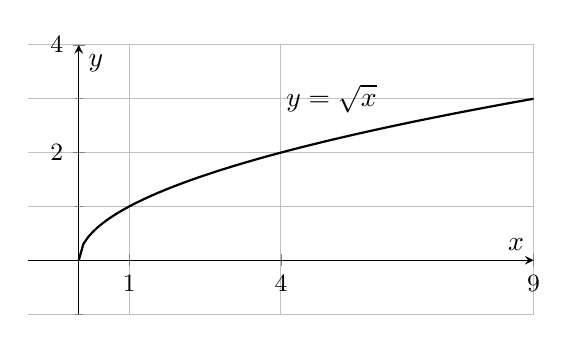
\begin{tikzpicture}\begin{axis}[coursaxe,xmin=-1,xmax=9,ymin=-1,ymax=4,width=8cm,height=5cm,xtick={0,1,4,9}]
\addplot[thick,domain=0:9]{sqrt(x)};\node at(axis cs:5,3){$y=\sqrt x$};\end{axis}\end{tikzpicture}
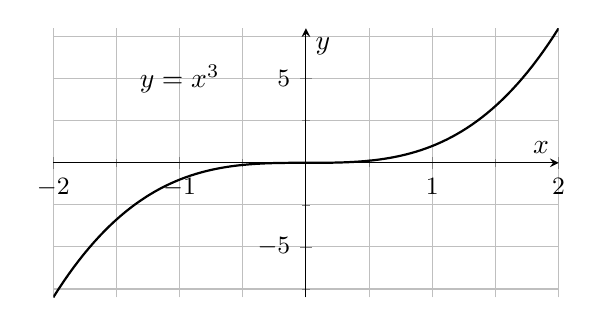
\begin{tikzpicture}\begin{axis}[coursaxe,xmin=-2,xmax=2,ymin=-8,ymax=8,width=8cm,height=5cm,xtick={-2,-1,0,1,2}]
\addplot[thick,domain=-2:2]{x*x*x};\node at(axis cs:-1,5){$y=x^3$};\end{axis}\end{tikzpicture}\end{center}
\ex{Solve $\sqrt x=3$; $\sqrt x=-2$; $\sqrt x\leq2$; $\sqrt x>3$; $x^3=-8$; $x^3\leq27$.}
\reponse[4]{$\{9\}$; $\varnothing$; $[0;4]$; $]9;+\infty[$; $\{-2\}$; $]-\infty;3]$. Respect the domain for square roots. The cube function preserves order.}
\ex{Compare $x^2$ and $x$ for $x=1/2$, then $x=2$. Is the square of a positive number always greater than the number itself?}
\reponse[2.4]{$1/4<1/2$ but $4>2$. The claim is false; $1/2$ is a counterexample. General study in sequence 10.}

\sequence{One-variable descriptive statistics}{Descriptive statistics}{7--18 December 2026}
\section{Frequencies, relative frequencies and mean}
\begin{cours}[Definitions]
A data set describes a characteristic over a population. If the value $x_i$ appears $n_i$ times, $n_i$ is its frequency count. The nonzero total count is $N=\sum_{i=1}^{p}n_i$; its relative frequency is $f_i=n_i/N$. The mean is
\[\overline x=\frac{\sum_{i=1}^{p}n_ix_i}{N}=\sum_{i=1}^{p}f_ix_i.\]
The range is $x_{\max}-x_{\min}$.
\end{cours}
\ex[Shoe sizes -- booklet data]{We study the shoe sizes of $30$ students:
\begin{center}\small\begin{tabular}{rrrrrrrrrrrrrrr}
36&42&40&41&41&38&39&43&42&42&42&40&36&40&39\\
41&40&38&44&42&40&42&43&38&43&36&41&41&44&43
\end{tabular}\end{center}
Complete the counts, calculate the relative frequencies, the mean and the range.}
\begin{center}\renewcommand{\arraystretch}{1.6}\begin{tabular}{c|rrrrrrrrr}
Size&36&37&38&39&40&41&42&43&44\\\hline
Count&\trou{3}&\trou{0}&\trou{3}&\trou{2}&\trou{5}&\trou{5}&\trou{6}&\trou{4}&\trou{2}
\end{tabular}\end{center}
\reponse[6]{Counts: $3,0,3,2,5,5,6,4,2$, with sum $30$. The relative frequencies are these counts divided by $30$, that is as percentages $10$; $0$; $10$; about $6.67$; $16.67$; $16.67$; $20$; $13.33$; $6.67$.
$\sum n_ix_i=1217$, so $\overline x=1217/30\approx40.57$. The range is $8$. The mean is not necessarily a value of the data set. The sum of the rounded percentages may differ slightly from $100$.}
\fiche{Median and cumulative counts}
\begin{cours}[Definition and convention]
A median is a number such that at least half of the values are less than or equal to it, and at least half are greater than or equal to it.
In the ordered data set of $N$ values, if $N$ is odd, take the value of rank $(N+1)/2$; if $N$ is even, choose the mean of the values of ranks $N/2$ and $N/2+1$.
\end{cours}
\vigilance{With repeated values, more than $50\,\%$ of the values can be less than or equal to the median.}
\ex{Complete the ascending cumulative counts (ACC) of the shoe sizes and determine the median.}
\begin{center}\renewcommand{\arraystretch}{1.7}\begin{tabular}{c|rrrrrrrrr}
Size&36&37&38&39&40&41&42&43&44\\\hline
Count&3&0&3&2&5&5&6&4&2\\
ACC&\trou{3}&\trou{3}&\trou{6}&\trou{8}&\trou{13}&\trou{18}&\trou{24}&\trou{28}&\trou{30}
\end{tabular}\end{center}
\reponse[4]{The central ranks are $15$ and $16$. The ACC goes from $13$ for $40$ to $18$ for $41$: both central values equal $41$, so $M_e=41$. At least half of the sizes are less than or equal to $41$, and at least half are greater than or equal to $41$.}
\ex{Calculate the medians of $1;2;2;8;9$ and of $1;2;8;9$.}
\reponse[3.2]{The third value of the first data set is $2$. In the second, $(2+8)/2=5$; the chosen median is not a value of the data set.}
\fiche{Quartiles and box plot}
\begin{cours}[Definitions]
The first quartile $Q_1$ is the value of rank $\lceil N/4\rceil$: the smallest value of the data set such that at least $25\,\%$ of the values are less than or equal to it. $Q_3$ is the value of rank $\lceil3N/4\rceil$.
The interquartile range is $Q_3-Q_1$. The box plot shows the minimum, $Q_1$, the median, $Q_3$ and the maximum.
\end{cours}
\ex{Determine $Q_1$, $Q_3$ and the interquartile range of the shoe sizes, then draw the box plot.}
\reponse[3.2]{$N/4=7.5$: rank $8$, so $Q_1=39$. $3N/4=22.5$: rank $23$, so $Q_3=42$. Interquartile range $3$. The plot uses $(36;39;41;42;44)$.}
\begin{center}\begin{tikzpicture}[x=1.5cm,y=1cm]
\draw[->](-.5,0)--(8.5,0);\foreach \x in {36,...,44}{\draw(\x-36,-.1)--(\x-36,.1)node[below=3pt]{$\x$};}
\ifprof\draw[thick](0,1)--(3,1)(6,1)--(8,1);\draw[thick](3,.5)rectangle(6,1.5);\draw[thick](5,.5)--(5,1.5)(0,.7)--(0,1.3)(8,.7)--(8,1.3);\else\path(0,1.8);\fi
\end{tikzpicture}\end{center}
\ex{Determine the quartiles of $1;2;2;3;4;4;4;5$. Are exactly $25\,\%$ of the values less than or equal to $Q_1$?}
\reponse[4]{$Q_1=2$ (rank $2$), $Q_3=4$ (rank $6$). Here $3/8=37.5\,\%$ of the values are less than or equal to $Q_1$. One must say ``at least''.}
\fiche{Adding or removing a value}
\begin{cours}[Properties]
Adding $a$ to a data set of size $N$ gives $\overline x'=(N\overline x+a)/(N+1)$.
Removing one occurrence of $a$, for $N>1$, gives $\overline x'=(N\overline x-a)/(N-1)$. Use the exact sum, with no intermediate rounding. Re-examine the median in the new ordered data set.
\end{cours}
\ex{In the shoe-size data, the sum is $1217$ and the median $41$.
\begin{enumerate}\item Add a size $36$ and calculate the new statistics.\item Starting again from the initial data, remove a size $44$ and repeat.\end{enumerate}}
\reponse[5]{1. Sum $1253$, count $31$: $\overline x'=1253/31\approx40.42$. The central rank $16$ still gives $41$. 2. Sum $1173$, count $29$: $\overline x''=1173/29\approx40.45$. The central rank $15$ gives $41$. The mean decreases in both cases; the median is unchanged. The situations are independent.}
\ex{Justify that adding the mean does not change the mean. Can the range decrease when a value is added?}
\reponse[4]{If $a=\overline x$, $(N\overline x+\overline x)/(N+1)=\overline x$. When adding, the minimum can only stay the same or decrease, the maximum stay the same or increase: the range does not decrease. When removing, it does not increase.}
\fiche{Variance and standard deviation}
\begin{cours}[Definitions]
$V=\dfrac{\sum n_i(x_i-\overline x)^2}{N}$ is the variance; $\sigma=\sqrt V$ is the standard deviation. It measures the spread around the mean and has the same unit as the data. One can also compute $V=\dfrac{\sum n_ix_i^2}{N}-\overline x^{\,2}$.
\end{cours}
\ex{Calculate the variance and the standard deviation of the shoe sizes.}
\reponse[4]{$\sum n_ix_i^2=49519$, so
\[V=\frac{49519}{30}-\left(\frac{1217}{30}\right)^2=\frac{4481}{900}\approx4.979.\]
$\sigma=\sqrt{4481}/30\approx2.23$. The standard deviation is not the maximum distance from the mean.}
\ex{Compare $A:8;10;12$ and $B:0;10;20$ using the mean--standard deviation pair and the median--interquartile range pair.}
\reponse[5]{The means and medians are all $10$. $V_A=8/3$, $\sigma_A\approx1.63$; $V_B=200/3$, $\sigma_B\approx8.16$. Quartiles: $8,12$ for $A$; $0,20$ for $B$. Interquartile ranges $4$ and $20$. $B$ is much more spread out despite identical centres.}
\prof{The descriptive variance divides by $N$, with no $N-1$ correction. Also check the quartile convention of software.}
\fiche{Linearity of the mean}
\begin{cours}[Property]
Replacing each $x_i$ by $kx_i+c$ gives a mean $k\overline x+c$, a standard deviation $|k|\sigma$ and a variance $k^2V$. Adding a constant changes neither variance nor standard deviation.
\end{cours}
\ex{Initial mean $12/20$, standard deviation $3$. Calculate the new statistics for three independent modifications, with no capping of marks: add $1.5$; multiply by $0.8$; multiply by $1.1$ then add $0.5$.}
\reponse[4]{Means: $13.5$, $9.6$, $13.7$. Standard deviations: $3$, $2.4$, $3.3$. Multiplying the marks by $1.1$ raises them; this does not mean making the assessment harder. With a cap at $20$, the transformation would no longer be affine on all the data.}
\begin{lstlisting}
from math import sqrt

def moyenne_ecart_type(valeurs):
    n = len(valeurs)
    if n == 0:
        raise ValueError("liste vide")
    m = sum(valeurs)/n
    v = sum((x-m)**2 for x in valeurs)/n
    return m, sqrt(v)
\end{lstlisting}
\ex{Explain the program; predict its result for \texttt{[8, 10, 12]}.}
\reponse[3.2]{It checks that the list is nonempty, calculates the mean, the mean of the squared deviations, then its root. Result: $(10;\sqrt{8/3})\approx(10;1.633)$.}
\fiche{Continuous data grouped into classes}
\begin{cours}[Definitions and loss of information]
A continuous quantitative variable can take every value in an interval. Here, the observations are grouped into classes of equal width; the centre of $[a;b[$ is $(a+b)/2$.
If the class means $m_i$ are known, the exact overall mean is $\sum n_im_i/N$. Otherwise, replacing them by the centres gives an estimate justified by a uniform model within each class.
\end{cours}
\ex[Heights -- booklet data]{Complete, estimate the mean from the centres and determine the median class.}
\begin{center}\renewcommand{\arraystretch}{1.7}\begin{tabular}{c|ccccc}
Class (cm)&$[150;160[$&$[160;170[$&$[170;180[$&$[180;190[$&$[190;200[$\\\hline
Count&8&22&35&28&7\\
Relative frequency (\%)&\trou{8}&\trou{22}&\trou{35}&\trou{28}&\trou{7}\\
Centre (cm)&\trou{155}&\trou{165}&\trou{175}&\trou{185}&\trou{195}\\
ACC&\trou{8}&\trou{30}&\trou{65}&\trou{93}&\trou{100}
\end{tabular}\end{center}
\reponse[4]{Width $10$ cm, total count $100$. Relative frequencies as percentages: $8,22,35,28,7$. Centres: $155,165,175,185,195$ cm. The weighted sum of the centres is $17540$, so the estimated mean is $175.4$ cm. The central ranks $50,51$ lie in $[170;180[$, the median class.}
\ex{If the exact class means were $154;166;174;184;196$ cm, what would the overall mean be?}
\reponse[2.4]{$(8\times154+22\times166+35\times174+28\times184+7\times196)/100=174.98$ cm.}
\fiche{Histogram and cumulative frequencies}
\begin{cours}[Representations]
The area of each rectangle of a histogram is proportional to the count. For equal widths, the heights can be the counts. The cumulative frequency polygon joins the points (upper bound; cumulative frequency), starting at the first lower bound with $0$.
\end{cours}
\ex{Construct both graphs for the heights of the previous example.}
\begin{center}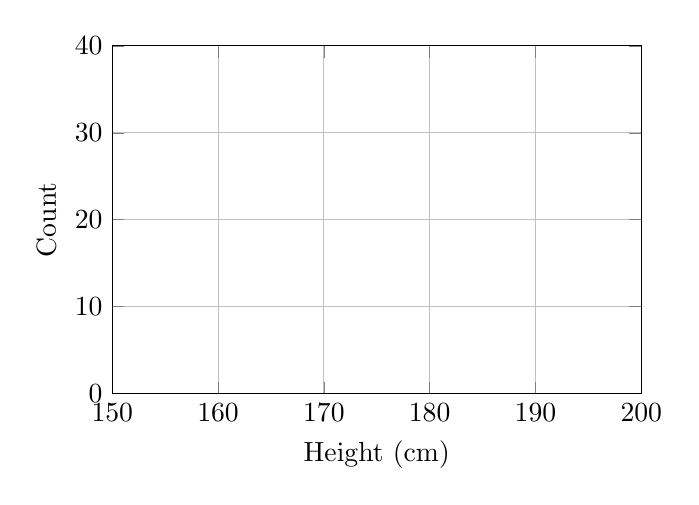
\begin{tikzpicture}\begin{axis}[width=8.3cm,height=6cm,xmin=150,xmax=200,ymin=0,ymax=40,xlabel={Height (cm)},ylabel={Count},xtick={150,160,...,200},ytick={0,10,20,30,40},grid=major]
\ifprof\addplot[ybar interval,fill=black!15,draw=black]coordinates{(150,8)(160,22)(170,35)(180,28)(190,7)(200,0)};\fi
\end{axis}\end{tikzpicture}
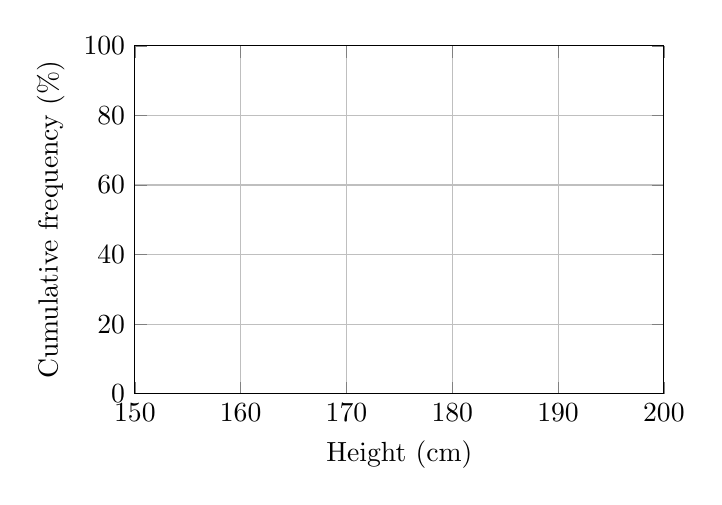
\begin{tikzpicture}\begin{axis}[width=8.3cm,height=6cm,xmin=150,xmax=200,ymin=0,ymax=100,xlabel={Height (cm)},ylabel={Cumulative frequency (\%)},xtick={150,160,...,200},ytick={0,20,...,100},grid=major]
\ifprof\addplot[thick,mark=*]coordinates{(150,0)(160,8)(170,30)(180,65)(190,93)(200,100)};\fi
\end{axis}\end{tikzpicture}\end{center}
\begin{methode}[Estimating the median]
Under the assumption of uniformity in $[170;180[$, the cumulative frequency rises linearly from $30\,\%$ to $65\,\%$. Look for the abscissa corresponding to $50\,\%$.
\end{methode}
\ex{Calculate this estimate and state its scope.}
\reponse[4]{Solve $(m-170)/10=(50-30)/(65-30)$, giving $m=170+10\times20/35\approx175.71$ cm. This is an estimate under an assumption of uniformity, not the exact median of the individual data. The class counts alone do not determine the latter.}

\sequence{Algebra, equations and inequalities}{Algebra}{4--20 January 2027}
\section{Brackets and distributivity}
\begin{methode}[Removing brackets]
After a $+$ sign, removing the brackets keeps the signs of the terms. After a $-$ sign, every term inside changes sign. This rule applies to a sum or a difference of terms.
\end{methode}
\ex{Remove the brackets and simplify: $A=x+(2+3x)$; $B=x-(2+3x)$; $C=-2x+(-4+5x)$; $D=-2x-(-4+5x)$.}
\reponse[3.2]{$A=4x+2$; $B=-2x-2$; $C=3x-4$; $D=-7x+4$.}
\begin{cours}[Distributivity]
For all real numbers $a,b,c,d$:
\[b(c+d)=bc+bd,\qquad(a+b)(c+d)=ac+ad+bc+bd.\]
\end{cours}
\ex{Expand and simplify:
\begin{align*}
A&=-4(8x+7)+(-8x+5)(5x+9),\\
B&=(6x+9)(-x+7)+(3x+5)(-9x+6),\\
C&=-9(-x-7)-(-x+3)(-8x-8),\\
D&=-5(-6x-7)+(x-7)(5x+8).
\end{align*}}
\reponse[5]{Expand each product, then collect terms of the same degree:
\begin{align*}
A&=-32x-28-40x^2-72x+25x+45=-40x^2-79x+17,\\
B&=-6x^2+33x+63-27x^2-27x+30=-33x^2+6x+93,\\
C&=9x+63-(8x^2-16x-24)=-8x^2+25x+87,\\
D&=30x+35+5x^2-27x-56=5x^2+3x-21.
\end{align*}}

\fiche{Factorising with a common factor}
\begin{cours}[Property]
$ka+kb=k(a+b)$ and $ka-kb=k(a-b)$. Factorising turns a sum into a product; expanding does the reverse.
\end{cours}
\ex{Factorise:
\begin{align*}
A&=15x^2-21x,\\B&=3(2+3x)-(5+2x)(2+3x),\\
C&=(4x-1)(x+6)+(4x-1),\\D&=(1-6x)^2-(1-6x)(2+5x).
\end{align*}}
\reponse[6]{
$A=3x(5x-7)$.\\
$B=(2+3x)[3-(5+2x)]=(2+3x)(-2-2x)=-2(2+3x)(1+x)$.\\
$C=(4x-1)[(x+6)+1]=(4x-1)(x+7)$.\\
$D=(1-6x)[(1-6x)-(2+5x)]=(1-6x)(-1-11x)=(6x-1)(11x+1)$.
Check the factors by expanding again.}
\ex{Choose a useful form of $f(x)=(x-2)(x+3)$ to calculate $f(2)$, $f(0)$ and find its zeros.}
\reponse[3.2]{The factorised form immediately gives $f(2)=0$ and the zeros $2,-3$. At $0$, $f(0)=(-2)\times3=-6$; the expanded form $x^2+x-6$ also gives this result. The choice depends on the question.}

\fiche{Special identities: expanding}
\begin{cours}[Identities]
\[(a+b)^2=a^2+2ab+b^2,\qquad(a-b)^2=a^2-2ab+b^2,\]
\[(a+b)(a-b)=a^2-b^2.\]
\end{cours}
\preuve[3.2]{Expand $(a+b)(a+b)$: $a^2+ab+ba+b^2=a^2+2ab+b^2$. Replacing $b$ by $-b$ gives the second identity. Finally $(a+b)(a-b)=a^2-ab+ab-b^2=a^2-b^2$.}
\ex{Expand $(x+3)^2$, $(3x-4)^2$, $(x-3)(x+3)$, $(2x+3)(2x-3)$, $(4-3x)(3x+4)$.}
\reponse[3.2]{$x^2+6x+9$; $9x^2-24x+16$; $x^2-9$; $4x^2-9$; $16-9x^2$. In the last product, reorder $3x+4$ as $4+3x$.}
\ex{Expand and simplify $A=(2x-3)^2+(x+5)(3-x)$ and $B=2(x+3)+(2x+3)(2x-3)$.}
\reponse[4]{$A=4x^2-12x+9-x^2-2x+15=3x^2-14x+24$. $B=2x+6+4x^2-9=4x^2+2x-3$.}

\fiche{Special identities: factorising}
\begin{methode}
Spot the two squares; for three-term forms, check the double product $2ab$. For a difference of two squares, use $a^2-b^2=(a-b)(a+b)$.
\end{methode}
\ex{Factorise:
\[A=x^2-2x+1,\quad B=25+16x^2-40x,\quad C=4x^2+12x+9,\]
\[D=1-49x^2,\quad E=9x^2-4,\quad F=(2x+3)^2-64.\]}
\reponse[6]{
$A=(x-1)^2$. $B=(4x-5)^2$. $C=(2x+3)^2$.\\
$D=(1-7x)(1+7x)$. $E=(3x-2)(3x+2)$.\\
$F=[(2x+3)-8][(2x+3)+8]=(2x-5)(2x+11)$.
For the first three, check the middle term; for $F$, treat $2x+3$ as a single block.}
\ex[Checking an identity]{Are the equalities $(a+b)^2=a^2+b^2$ and $a^2+b^2=(a-b)(a+b)$ true for all real numbers?}
\reponse[3.2]{No: for $a=b=1$, the first would give $4=2$ and the second $2=0$. The missing term in the first is $2ab$; the product in the second equals $a^2-b^2$.}
\rituel{Calculate $101^2$ mentally; give a direction vector of $2x+3y=1$; determine $[-1;3]\cap[2;5]$.}{$10201$; $(-3;2)$; $[2;3]$.}

\fiche{Integer powers}
\begin{cours}[Definition and rules]
For $n\geq1$, $a^n$ is the product of $n$ factors equal to $a$. For $a\ne0$, $a^0=1$ and $a^{-n}=1/a^n$. In this course, $0^0$ is not defined.
For $a,b\ne0$ and integers $m,n$:
\[a^ma^n=a^{m+n},\quad\frac{a^m}{a^n}=a^{m-n},\quad(a^m)^n=a^{mn},\]
\[(ab)^n=a^nb^n,\qquad\left(\frac ab\right)^n=\frac{a^n}{b^n}.\]
For strictly positive exponents, some bases may be zero if the expressions remain defined.
\end{cours}
\ex{Simplify $A=2^4\times2^3$, $B=(-5)^{12}/(-5)^3$, $C=(7^3)^6\times7^{-5}$, $D=7^{24}\times3^2\times2^3$. Also calculate $(-3)^5$, $5^1$ and $99999^0$.}
\reponse[4]{$A=2^7=128$. $B=(-5)^9=-1953125$. $C=7^{18-5}=7^{13}$. $D=72\times7^{24}$: exponents of different bases cannot be added. The last three values are $-243$, $5$, $1$.}
\vigilance{The definition as a repeated product does not hold for a negative exponent. $-3^2=-9$, whereas $(-3)^2=9$.}
\ex{Solve $2^n>100$ mentally for the smallest natural number $n$. Write a program that finds it.}
\reponse[4]{$2^6=64\leq100<128=2^7$, so $n=7$. Initialise $n=0$, $p=1$; while $p\leq100$, replace $p$ by $2p$ and $n$ by $n+1$. The program is given at the end of the sequence.}

\fiche{Fractions and fractional expressions}
\begin{cours}[Rules and conditions]
For nonzero denominators:
\[\frac ac\pm\frac bc=\frac{a\pm b}{c},\quad\frac ac\pm\frac bd=\frac{ad\pm bc}{cd},\quad\frac ac\times\frac bd=\frac{ab}{cd}.\]
A fraction $c/d$ has an inverse only if $c\ne0$ and $d\ne0$. Then
\[\frac ab\div\frac cd=\frac ab\times\frac dc=\frac{ad}{bc}\quad(b,c,d\ne0).\]
\end{cours}
\ex{Calculate and reduce to lowest terms:
\[A=\left(\frac23+\frac16\right)\times\frac45,\quad B=\frac12+\frac34\times\frac56,\quad C=\frac45\div\frac23\times\frac7{10},\]
\[D=\frac{\left(\frac25+\frac13\right)\times\frac34}{\frac12-\frac16}.\]}
\reponse[5]{$A=\frac56\times\frac45=\frac23$. $B=\frac12+\frac58=\frac98$. $C=\frac45\times\frac32\times\frac7{10}=\frac{21}{25}$. $D=\frac{11}{15}\times\frac34\div\frac13=\frac{11}{20}\times3=\frac{33}{20}$. In $C$, multiplication and division are carried out from left to right.}
\ex{Simplify $\dfrac{x^2-1}{x-1}$, stating the domain. Can we then take $x=1$?}
\reponse[3.2]{For $x\ne1$, $\frac{(x-1)(x+1)}{x-1}=x+1$. The original expression remains undefined at $1$; the simplification does not lift the restriction.}

\fiche{Square roots and validity conditions}
\begin{cours}[Definition and properties]
For $a\geq0$, $\sqrt a$ is the unique positive or zero number whose square is $a$. Thus $(\sqrt a)^2=a$. For every $x\in\R$, $\sqrt{x^2}=|x|$.
For $a,b\geq0$, $\sqrt{ab}=\sqrt a\sqrt b$. If $b>0$, $\sqrt{a/b}=\sqrt a/\sqrt b$.
\end{cours}
\preuve[3.2]{The number $\sqrt a\sqrt b$ is positive or zero and its square is $ab$; by uniqueness of the positive square root, it equals $\sqrt{ab}$. The same argument applied to the quotient establishes the second formula, under $b>0$. Similarly $|x|\geq0$ and $|x|^2=x^2$, so $\sqrt{x^2}=|x|$.}
\ex{Simplify $\sqrt{18}$; $\sqrt2\sqrt8$; $\sqrt{7/25}$; $\sqrt{27/75}$; $\sqrt{(-5)^2}$.}
\reponse[3.2]{$3\sqrt2$; $4$; $\sqrt7/5$; $\sqrt{9/25}=3/5$; $5$.}
\vigilance{There is no general rule $\sqrt{a+b}=\sqrt a+\sqrt b$. With $a=4,b=9$, we would wrongly have $\sqrt{13}=5$. Saying these expressions are always different would also be wrong, for example if $a=0$.}
\ex{Simplify $2\sqrt{18}-\sqrt{50}+\sqrt8$. Bound $\sqrt{20}$ between two consecutive integers.}
\reponse[3.2]{$6\sqrt2-5\sqrt2+2\sqrt2=3\sqrt2$. Since $16<20<25$, $4<\sqrt{20}<5$.}

\fiche{First-degree equations}
\begin{cours}[Definition]
To solve an equation is to find all the values of the unknown that satisfy the equality. Two equations are equivalent if they have the same solutions. Adding the same expression or multiplying by the same nonzero number preserves equivalence.
\end{cours}
\begin{methode}
Expand if necessary, collect the terms in $x$, then isolate $x$. If its coefficient is zero, examine the remaining equality: it may be always true or impossible. Check in the original equation.
\end{methode}
\ex{Solve:
\begin{align*}
a)&\ 5x-3=2x+9,& b)&\ 3(2x-1)=2(x+4)+7,\\
c)&\ -2(x+3)=4x-(x-1),&d)&\ \frac{x+2}{3}=x-1,\\
e)&\ \frac{-5x+5}{8}=-\frac34,&f)&\ \frac{-3x-1}{9}=-\frac74.
\end{align*}}
\reponse[6]{a) $3x=12$, so $x=4$. b) $6x-3=2x+15$, so $x=9/2$. c) $-2x-6=3x+1$, so $x=-7/5$. d) $x+2=3x-3$, so $x=5/2$. e) $-5x+5=-6$, so $x=11/5$. f) $4(-3x-1)=-63$, so $-12x=-59$ and $x=59/12$.}
\ex{Solve $2(x+1)=2x+2$, then $2(x+1)=2x+3$.}
\reponse[2.4]{The first reduces to $2=2$: $S=\R$. The second gives $2=3$: $S=\varnothing$. We do not divide by a zero coefficient.}

\fiche{Zero-product property and equations with a quotient}
\begin{cours}[Properties]
$AB=0\iff A=0$ or $B=0$. For $B\ne0$, $A/B=0\iff A=0$. To solve $A(x)/B(x)=k$, first require $B(x)\ne0$, then solve $A(x)=kB(x)$ and discard the forbidden values.
\end{cours}
\ex{Solve $(4x+6)(3-7x)=0$; $3x(-7x+5)=0$; $\dfrac{2x+1}{3x-5}=0$.}
\reponse[3.2]{Solutions: $\{-3/2;3/7\}$; $\{0;5/7\}$; $\{-1/2\}$, with forbidden value $5/3$ in the last case.}
\ex{Factorise then solve $(1-6x)^2-(1-6x)(2+5x)=0$ and $(4x-1)(x+6)+(4x-1)=0$.}
\reponse[3.2]{First: $(6x-1)(11x+1)=0$, so $S=\{1/6;-1/11\}$. Second: $(4x-1)(x+7)=0$, so $S=\{1/4;-7\}$.}
\ex{Solve $\dfrac{x+1}{x-2}=3$, then $\dfrac{x^2-4}{x-2}=4$.}
\reponse[4]{In both cases, $x\ne2$. First: $x+1=3x-6$, so $x=7/2$, allowed. Second: for $x\ne2$, the quotient equals $x+2$; the equation requires $x=2$, forbidden. So no solution.}

\fiche{Equations with a square; isolating a variable}
\begin{cours}[Reminder]
In $\R$, $x^2=a$ has two solutions $\pm\sqrt a$ if $a>0$, one solution $0$ if $a=0$, and none if $a<0$.
\end{cours}
\ex{Solve $x^2=0$; $x^2=-8$; $x^2=7$; $25x^2=81$; $(x+2)^2=9$.}
\reponse[4]{In order: $\{0\}$; $\varnothing$; $\{-\sqrt7;\sqrt7\}$; $\{-9/5;9/5\}$; $\{-5;1\}$. For the last one, $x+2=-3$ or $x+2=3$.}
\begin{methode}[Isolating a variable in a formula]
Describe the operations performed on both sides; state the conditions that allow dividing or taking a square root.
\end{methode}
\ex{Isolate $h$ in $V=\pi r^2h$ with $r>0$; isolate $v$ in $E=\frac12mv^2$ with $m>0$, $E\geq0$ and $v\geq0$; isolate $x$ in $y=ax+b$ with $a\ne0$.}
\reponse[4]{$h=V/(\pi r^2)$. Then $v^2=2E/m$; since $v\geq0$, $v=\sqrt{2E/m}$. Finally $x=(y-b)/a$. Without the condition $v\geq0$, two signs would be possible for $E>0$.}
\rituel{Give the domain of $1/(x+3)$; calculate $\sqrt{49}$; the slope between $(0;2)$ and $(3;8)$.}{$\R\setminus\{-3\}$; $7$; $2$.}

\fiche{Inequalities and comparison}
\begin{cours}[Rules]
Inequalities of the same direction can be added: $a\leq b$, $c\leq d\Rightarrow a+c\leq b+d$. Adding the same real number preserves the direction. Multiplying or dividing by a strictly positive real number preserves the direction; by a strictly negative one, it reverses it.
Comparing $A$ and $B$ amounts to studying the sign of $A-B$. If $A,B>0$, one can also compare $A/B$ to $1$.
\end{cours}
\ex{1. If $x\leq-4$, what can be said about $3x-4$? 2. If $x>-6$, what can be said about $2x-3$? 3. If $7\leq x\leq16$ and $3\leq y\leq12$, bound $8x+7y$. 4. If $-10\leq x\leq-6$, bound $2x-6$.}
\reponse[4]{1. $3x-4\leq-16$. 2. $2x-3>-15$. 3. $56\leq8x\leq128$ and $21\leq7y\leq84$, so $77\leq8x+7y\leq212$. The bounds are attainable. 4. $-26\leq2x-6\leq-18$.}
\ex{Solve $3x+1\geq x-7$; $2x-11\leq4x-5$; $6x+19\leq2x-3$.}
\reponse[4]{1. $2x\geq-8$, that is $[-4;+\infty[$. 2. $-6\leq2x$, that is $[-3;+\infty[$. 3. $4x\leq-22$, that is $]-\infty;-11/2]$.}

\fiche{Sign of an affine expression and of a product}
\begin{cours}[Property]
For $a\ne0$, $ax+b$ vanishes at $x_0=-b/a$; its sign to the right is that of $a$, to the left the opposite. If $a=0$, the sign is that of the constant $b$. For a product, multiply the signs of the factors.
\end{cours}
\ex{Draw the sign tables of $3-x$, $2x-6$, then $P(x)=(2x-6)(x+1)$.}
\reponse[5]{Both affine expressions vanish at $3$: $3-x$ is positive on the left, negative on the right; $2x-6$ has the opposite signs.
\begin{center}\renewcommand{\arraystretch}{1.5}\begin{tabular}{c|ccccccc}
$x$&$-\infty$&&$-1$&&$3$&&$+\infty$\\\hline
$2x-6$&&$-$&$-$&$-$&$0$&$+$&\\
$x+1$&&$-$&$0$&$+$&$+$&$+$&\\\hline
$P(x)$&&$+$&$0$&$-$&$0$&$+$&
\end{tabular}\end{center}}
\ex{Solve $(7+3x)(2x+6)>0$.}
\reponse[5]{The zeros are $-7/3$ and $-3$, to be ordered $-3<-7/3$. The product is positive outside these roots and negative between them. The inequality is strict: $S=]-\infty;-3[\cup]-7/3;+\infty[$.}

\fiche{Sign of a quotient and algorithmic synthesis}
\begin{methode}
Find the forbidden values, then the zeros of the numerator. Order all the critical values and apply the sign rule. On the quotient row, a double bar indicates a forbidden value.
\end{methode}
\ex{Draw the sign table of $Q(x)=\dfrac{-4x+6}{x-3}$, then solve $\dfrac{2x-1}{-4x+3}\leq0$.}
\reponse[5]{For $Q$, zero $3/2$, forbidden $3$. Signs: negative on $]-\infty;3/2[$, zero at $3/2$, positive on $]3/2;3[$, undefined at $3$, negative on $]3;+\infty[$.
For the second expression, zero $1/2$, forbidden $3/4$. The signs are $-,+,-$ on the three intervals. Thus $S=]-\infty;1/2]\cup]3/4;+\infty[$.}
\begin{lstlisting}
def premiere_puissance(seuil):
    # seuil reel >= 1
    n, p = 0, 1
    while p <= seuil:
        n = n+1
        p = 2*p
    return n, p
\end{lstlisting}
\ex{What does \texttt{premiere\_puissance(100)} return? What relation between \texttt{p} and \texttt{n} stays true at each step? How can the sign of a number then be tested in Python?}
\reponse[3.2]{The result is $(7,128)$. The invariant is $p=2^n$, true at initialisation and then preserved. For the sign, first test \texttt{x > 0}, then \texttt{x < 0}, otherwise $x=0$. Do not replace the loop's non-strict inequality by a strict one without changing the problem posed.}

\sequence{Proportions and percentage change}{Proportions and percentage change}{21--29 January 2027}
\section{Proportion and proportion of a proportion}
\begin{cours}[Definitions]
In a nonempty finite set $E$, the proportion of a subset $F$ is $p=\Card(F)/\Card(E)$; $0\leq p\leq1$. Its expression as a percentage is $100p\,\%$.
If $G\subseteq F\subseteq E$, $F\ne\varnothing$, and if $p_1$ is the proportion of $F$ in $E$ and $p_2$ that of $G$ in $F$, the proportion of $G$ in $E$ is $p_1p_2$.
\end{cours}
\ex{A school has $1500$ students, of whom $652$ are day boarders. Calculate their proportion. In a class, $60\,\%$ of the students play sport; among them, $40\,\%$ are boys. What proportion of the class do the boys who play sport represent?}
\reponse[4]{$652/1500\approx0.4347$, that is about $43.47\,\%$. For the class, $0.60\times0.40=0.24$, that is $24\,\%$. The second percentage has the sporty students as its reference, not the whole class.}
\ex{In a fictional school of $800$ students, $35\,\%$ play a sport at a club; among them, $45\,\%$ play a team sport. Calculate the two counts and the final proportion.}
\reponse[4]{$800\times0.35=280$ students at a club. $280\times0.45=126$ in a team sport. The final proportion is $126/800=0.1575=15.75\,\%$.}
\vigilance{Proportion and rate of change do not answer the same question: a proportion compares a part to a whole, a rate compares a change to an initial value.}

\fiche{Absolute change and rate of change}
\begin{cours}[Definition]
For an initial value $V_I>0$ and a final value $V_F>0$, the absolute change is $V_F-V_I$; the rate of change is
\[t=\frac{V_F-V_I}{V_I}.\]
The rate has no unit. It is positive for an increase, negative for a decrease. The reference is always the initial value.
\end{cours}
\ex{A cheese is sold for $2.13$ euros instead of $3.55$ euros. Calculate the absolute change and the rate.}
\reponse[3.2]{Absolute change: $2.13-3.55=-1.42$ euro. Rate: $-1.42/3.55=-0.40$, that is a decrease of $40\,\%$.}
\begin{cours}[Multiplier]
$CM=V_F/V_I=1+t$, so $V_F=V_I(1+t)$. To recover $V_I$, divide $V_F$ by $1+t$ (nonzero).
\end{cours}
\ex{A fictional item priced $50000$ Ar increases by $12\,\%$, then separately consider a $12\,\%$ discount on the initial price. Give the final prices. A price after a $20\,\%$ increase is $72000$ Ar; find its initial price.}
\reponse[4]{Increase: $50000\times1.12=56000$ Ar. Discount: $50000\times0.88=44000$ Ar. Last question: $V_I=72000/1.20=60000$ Ar.}
\rituel{Expand $(x-3)^2$; solve $1/x=5$; give the mean of $8;10;12$.}{$x^2-6x+9$; $x=1/5$; $10$.}

\fiche{Successive changes}
\begin{cours}[Property]
Successive changes with rates $t_1,t_2$ have overall multiplier
\[CM_G=(1+t_1)(1+t_2),\qquad t_G=(1+t_1)(1+t_2)-1.\]
We multiply the multipliers; we do not simply add the rates.
\end{cours}
\ex{A manufacturer sold $5600$ bicycles in 2022, which is $25\,\%$ more than in 2021. Its sales decrease by $15\,\%$ in 2023. Determine the sales of 2021 and 2023, then the overall rate between these two years.}
\reponse[4]{2021: $5600/1.25=4480$ bicycles. 2023: $5600\times0.85=4760$ bicycles. Overall multiplier $1.25\times0.85=1.0625$, so an overall increase of $6.25\,\%$. Check: $(4760-4480)/4480=0.0625$.}
\ex{A price increases by $10\,\%$ then decreases by $10\,\%$. Does it return to the initial price?}
\reponse[3.2]{$CM_G=1.10\times0.90=0.99$. The final price is $99\,\%$ of the initial price: an overall decrease of $1\,\%$. The two rates refer to different reference values.}
\ex{A rate goes from $20\,\%$ to $25\,\%$. Explain the difference between the increase in percentage points and the relative change.}
\reponse[3.2]{The gap is $5$ percentage points. The relative change is $(0.25-0.20)/0.20=0.25$, that is an increase of $25\,\%$.}

\fiche{Reverse change}
\begin{cours}[Property]
To return to the initial value after a change of rate $t>-1$, use the multiplier $1/(1+t)$. The reverse rate is
\[t_{\text{reverse}}=\frac1{1+t}-1=\frac{-t}{1+t}.\]
\end{cours}
\ex{Which rate compensates a $25\,\%$ increase? Which rate compensates a $20\,\%$ decrease?}
\reponse[4]{After a $25\,\%$ increase, the reverse multiplier is $1/1.25=0.8$: a $20\,\%$ decrease. After a $20\,\%$ decrease, it is $1/0.8=1.25$: a $25\,\%$ increase.}
\ex{A price undergoes a $30\,\%$ discount, then a $10\,\%$ increase. What additional percentage increase restores the initial price?}
\reponse[5]{The current multiplier is $0.70\times1.10=0.77$. The required multiplier is $1/0.77=100/77$. The rate is $23/77\approx0.2987$, that is about $29.87\,\%$. Check $0.77\times(100/77)=1$.}
\prof{Have students state the base of the percentage at each step. The reverse-rate formula is justified by a product equal to $1$; memorisation alone is fragile.}

\sequence{Variations and extrema of a function}{Variations and extrema}{1--12 February 2027}
\section{Increasing, decreasing and monotonicity}
\begin{cours}[Definitions]
On an interval $I$, $f$ is increasing if for all $a,b\in I$, $a<b\Rightarrow f(a)\leq f(b)$; decreasing if $a<b\Rightarrow f(a)\geq f(b)$. The variations are strict when the inequalities between images are strict. A constant function has the same value everywhere; it is both increasing and decreasing in the broad sense.
A function that is monotonic on $I$ is increasing or decreasing there.
\end{cours}
\begin{methode}[Table of variations]
Indicate the domain, the intervals of monotonicity, the values at the endpoints when defined, then the arrows. A sign table shows whether $f(x)$ is positive or negative; a table of variations shows how its values change.
\end{methode}
\ex{On $[-3;4]$, $f(x)=(x-1)^2-2$. Using the square, extending the curve studied in sequence 6, draw its table of variations. Give two numbers $a<b$ such that $f(a)>f(b)$.}
\reponse[5]{The function decreases strictly on $[-3;1]$, then increases strictly on $[1;4]$. $f(-3)=14$, $f(1)=-2$, $f(4)=7$.
\[\begin{array}{c|ccccc}x&-3&&1&&4\\\hline f(x)&14&\searrow&-2&\nearrow&7\end{array}\]
For example $a=0<b=1$ and $f(0)=-1>-2=f(1)$.}
\ex{Can a function be negative and increasing? Give an example on an interval.}
\reponse[3.2]{Yes: $f(x)=x-5$ on $[0;2]$ is strictly increasing and stays between $-5$ and $-3$, so it is strictly negative.}

\fiche{Maximum and minimum on an interval}
\begin{cours}[Definitions]
$f$ has a maximum at $a\in I$ if, for every $x\in I$, $f(x)\leq f(a)$. The value of the maximum is $f(a)$.
$f$ has a minimum at $b\in I$ if, for every $x\in I$, $f(x)\geq f(b)$.
An extremum must be attained. Distinguish its value from the abscissa where it is attained.
\end{cours}
\ex{Return to $f(x)=(x-1)^2-2$ on $[-3;4]$. Give the minimum and maximum, then where they are attained. Repeat on $[0;4]$.}
\reponse[4]{On $[-3;4]$, minimum $-2$ at $x=1$, maximum $14$ at $x=-3$. On $[0;4]$, the minimum remains $-2$ at $1$, but the maximum is $7$ at $4$. The maximum depends on the domain.}
\ex{Does the function $f(x)=x$ have a maximum on $[0;1[$? A minimum?}
\reponse[3.2]{It has minimum $0$, attained at $0$. It has no maximum: for every $x<1$, $(x+1)/2$ still belongs to $[0;1[$ and has a larger image. The number $1$ is an upper bound, but is not attained.}
\begin{cours}[Reading without inventing]
A table of variations does not provide all the intermediate images. It allows comparing certain images; if the abscissae lie on different branches, the comparison may be indeterminate.
\end{cours}
\ex{Does the mere fact that a function decreases then increases allow comparing two images on either side of the minimum?}
\reponse[2.4]{No. Additional information is needed. For $x\mapsto x^2$, the images of $-2$ and $1$ are $4$ and $1$, while those of $-1$ and $2$ are $1$ and $4$.}

\fiche{Variations of affine functions}
\begin{cours}[Property and rate of change]
For $f(x)=mx+p$ and $a\ne b$,
\[\frac{f(b)-f(a)}{b-a}=m.\]
If $m>0$, $f$ is strictly increasing; if $m<0$, strictly decreasing; if $m=0$, constant.
\end{cours}
\preuve[4]{For $a<b$, $f(b)-f(a)=m(b-a)$. Since $b-a>0$, the difference has the sign of $m$. It is positive, negative or zero according to the three cases, which gives the stated variations. Dividing by $b-a$ gives the constant rate of change.}
\ex{Determine the variations of $f(x)=3x+2$, $g(x)=7-6x$, $h(x)=-x$. Give the sign of $2x-6$ and explain why the sign of this function does not stay constant although it is increasing.}
\reponse[4]{$f$ is strictly increasing; $g,h$ strictly decreasing. $2x-6$ is negative for $x<3$, zero at $3$, positive for $x>3$. An increasing function can cross $0$; its direction of variation does not determine a single sign.}
\ex{An affine function $u$ satisfies $u(2)=5$, $u(6)=13$. Determine $u$, then its minimum and maximum on $[-1;4]$.}
\reponse[3.2]{$m=(13-5)/(6-2)=2$, $p=1$, so $u(x)=2x+1$. It is increasing: minimum $u(-1)=-1$, maximum $u(4)=9$.}

\fiche{Variations of the square and the absolute value}
\begin{cours}[Properties]
$x\mapsto x^2$ and $x\mapsto|x|$ are strictly decreasing on $]-\infty;0]$ and strictly increasing on $[0;+\infty[$. Their minimum on $\R$ is $0$, attained only at $0$.
\end{cours}
\preuve[5]{For $a<b$, $b^2-a^2=(b-a)(a+b)$. If $0\leq a<b$, both factors are strictly positive: $a^2<b^2$. If $a<b\leq0$, the first factor is positive and the second negative: $a^2>b^2$.
For the absolute value, on $[0;+\infty[$, $|x|=x$ is increasing; on $]-\infty;0]$, $|x|=-x$ is decreasing. Positivity and vanishing at $0$ give the minimum.}
\ex{Compare without a calculator: $(-3.2)^2$ and $(-3.1)^2$; $1.2^2$ and $1.3^2$; $|-5|$ and $|-2|$.}
\reponse[3.2]{On the negatives, the square reverses the order: $(-3.2)^2>(-3.1)^2$. On the positives, $1.2^2<1.3^2$. Finally $|-5|>|-2|$, that is $5>2$.}
\ex{Bound $x^2$ if $-3\leq x\leq2$. Why can we not simply square the two bounds?}
\reponse[3.2]{The minimum is $0$ and the maximum $9$: $0\leq x^2\leq9$. The square is not monotonic on $[-3;2]$. Squaring only the bounds would wrongly give $9\leq x^2\leq4$.}

\fiche{Variations of the inverse function}
\begin{cours}[Property]
The inverse function is strictly decreasing on $]-\infty;0[$ and on $]0;+\infty[$, separately. It is not decreasing on the whole of $\R^*$.
\end{cours}
\preuve[4]{For $a<b$ of the same sign, $ab>0$ and
\[\frac1b-\frac1a=\frac{a-b}{ab}<0.\]
So $1/b<1/a$. On the other hand, $-1<1$ and $1/(-1)=-1<1=1/1$: the decreasing criterion fails on the whole of $\R^*$.}
\ex{Compare $1/(-4)$ and $1/(-2)$, then $1/3$ and $1/5$. Bound $1/x$ if $2\leq x\leq5$, then if $-5\leq x\leq-2$.}
\reponse[4]{$-1/4>-1/2$; $1/3>1/5$. For $x\in[2;5]$, $1/5\leq1/x\leq1/2$. For $x\in[-5;-2]$, $-1/2\leq1/x\leq-1/5$.}
\ex{Why is the interval $[-1;1]$ not suitable for directly applying a variation rule of the inverse function?}
\reponse[3.2]{The function is not defined at $0$, which belongs to the interval. One must work on the two parts of the domain; moreover, the comparison behaviour of the function is not the same when crossing $0$.}

\fiche{Relative position of a number and its square}
\begin{cours}[Property on the positives]
For $0\leq x\leq1$, $x^2\leq x$; for $x\geq1$, $x^2\geq x$. Equality holds at $0$ and $1$.
\end{cours}
\preuve[3.2]{$x^2-x=x(x-1)$. On $[0;1]$, the first factor is positive or zero, the second negative or zero: their product is negative or zero. On $[1;+\infty[$, both are positive or zero. The product is zero if $x=0$ or $x=1$.}
\begin{cours}[Square root and cube]
The square root function is strictly increasing on $[0;+\infty[$. The cube function is strictly increasing on $\R$.
\end{cours}
\ex{Explain why the square root is increasing from the increase of the square on the positives. For the cube, use $b^3-a^3=(b-a)(a^2+ab+b^2)$.}
\reponse[4]{If $0\leq a<b$ but $\sqrt a\geq\sqrt b$, the increase of the square on the positives would give $a\geq b$, a contradiction. For $a<b$, $b-a>0$ and $a^2+ab+b^2=(a+b/2)^2+3b^2/4>0$ (equality would require $a=b=0$). So $b^3-a^3>0$.}
\ex{Compare $\sqrt{5}$ and $\sqrt6$, then $(-2)^3$ and $(-1)^3$.}
\reponse[2.4]{$\sqrt5<\sqrt6$ and $-8<-1$, consistent with the two increasing behaviours.}

\fiche{Optimising: conjecture and prove}
\ex{A rectangle of perimeter $20$ m has area $A(x)=x(10-x)$ with $x\in]0;10[$.
\begin{enumerate}\item Conjecture the maximum area using a table of values.\item Show that $A(x)=25-(x-5)^2$. Deduce the exact maximum and the corresponding dimensions.\end{enumerate}}
\reponse[4]{For $x=1,2,3,4,5,6,7,8,9$, the areas are $9,16,21,24,25,24,21,16,9$ m$^2$. Expanding, $25-(x-5)^2=10x-x^2=A(x)$. Since $(x-5)^2\geq0$, $A(x)\leq25$, with equality only at $x=5$. The optimal rectangle is a square of side $5$ m.}
\begin{lstlisting}
def aire(x):
    return x*(10-x)

def maximum_grille(N):
    # N entier >= 2 ; points strictement entre 0 et 10
    meilleur_x = 10/N
    meilleur_y = aire(meilleur_x)
    for k in range(2, N):
        x = 10*k/N
        if aire(x) > meilleur_y:
            meilleur_x, meilleur_y = x, aire(x)
    return meilleur_x, meilleur_y
\end{lstlisting}
\ex{What does the program return for $N=10$? Does a numerical sweep always prove the maximum of a function on an interval?}
\reponse[3.2]{For $N=10$, $(5,25)$. The program finds the maximum only over the sampled points. It can miss a maximum between two points: the algebraic proof gives the exact result here. An ordinary bisection for finding a zero does not automatically apply to finding an extremum.}

\sequence{Cross-tabulating two qualitative variables}{Two-way tables}{1--12 March 2027}
\section{Two-way tables and marginal frequencies}
\begin{cours}[Definitions]
A qualitative variable describes a category. It is nominal if its categories have no natural order (means of transport), ordinal if they are ordered (level of satisfaction).
A two-way table counts individuals according to two variables. The sums of the rows and columns are the margins. A marginal frequency divides a margin by the total count.
\end{cours}
\ex{In a population of $100$ individuals, two characteristics $A,B$ are observed:}
\begin{center}\renewcommand{\arraystretch}{1.6}\begin{tabular}{c|rr|r}
&$A$&$\overline A$&Total\\\hline
$B$&20&15&35\\
$\overline B$&12&53&65\\\hline
Total&32&68&100
\end{tabular}\end{center}
Calculate the marginal frequencies of $A$, $B$, $\overline B$, then the frequency of individuals satisfying both $A$ and $B$.
\reponse[2]{$f(A)=32/100=0.32$; $f(B)=35/100=0.35$; $f(\overline B)=65/100=0.65$. The frequency of $A\cap B$ is $20/100=0.20$; it is not a marginal frequency.}
\ex{A Year 12 class of $32$ students is split as follows. Complete the margins and calculate the marginal frequencies ``CS'' and ``girls''.}
\begin{center}\renewcommand{\arraystretch}{1.5}\begin{tabular}{c|rr|r}
&Boys&Girls&Total\\\hline
CS&12&9&\trou{21}\\
No CS&6&5&\trou{11}\\\hline
Total&\trou{18}&\trou{14}&32
\end{tabular}\end{center}
\reponse[1.6]{$f(\mathrm{CS})=21/32=65.625\,\%$; $f(\mathrm{girls})=14/32=43.75\,\%$.}

\fiche{Conditional frequencies and reading sentences}
\begin{cours}[Definition]
The frequency of $A$ \textbf{among the individuals of $B$}, if this subpopulation is nonempty, is
\[f_B(A)=\frac{\text{count satisfying }A\text{ and }B}{\text{count of }B}.\]
The denominator corresponds to the population introduced by ``among''.
\end{cours}
\ex{In the CS table, calculate the frequency of girls among the students without CS, then the frequency of students without CS among the girls. Are the two results equal?}
\reponse[4]{Among the $11$ students without CS, $5$ are girls: $5/11\approx45.45\,\%$. Among the $14$ girls, $5$ do not take CS: $5/14\approx35.71\,\%$. The numerator is the same, the reference populations differ.}
\ex{In the table of $100$ individuals, calculate $f_B(A)$, $f_A(B)$ and $f_{\overline A}(B)$. Translate each result into a sentence.}
\reponse[4]{$f_B(A)=20/35=4/7\approx57.14\,\%$ of the individuals of $B$ satisfy $A$. $f_A(B)=20/32=62.5\,\%$ of the individuals of $A$ satisfy $B$. $f_{\overline A}(B)=15/68\approx22.06\,\%$ of the individuals not satisfying $A$ satisfy $B$.}
\ex{Does ``$60\,\%$ of cyclists are students'' allow us to conclude that $60\,\%$ of students are cyclists?}
\reponse[2.4]{No. For example, out of $10$ cyclists, $6$ are students; if the population has $100$ students in all, only $6\,\%$ of the students are cyclists.}

\fiche{Completing a table from frequencies}
\ex[Fictional situation]{A group has $200$ people, of whom $120$ use a bus ($B$). Among these $120$ people, $75\,\%$ have a pass ($A$). Among the other $80$, $25\,\%$ have a pass.
\begin{enumerate}\item Construct the two-way table $B/\overline B$ and $A/\overline A$ with its margins.\item Calculate the marginal frequency of $A$.\item Calculate the frequency of $B$ among $A$.\end{enumerate}}
\reponse[6]{In $B$, $120\times0.75=90$ people satisfy $A$, so $30$ do not. In $\overline B$, $80\times0.25=20$ satisfy $A$, and $60$ do not.
\begin{center}\begin{tabular}{c|rr|r}&$A$&$\overline A$&Total\\\hline $B$&90&30&120\\$\overline B$&20&60&80\\\hline Total&110&90&200\end{tabular}\end{center}
$f(A)=110/200=55\,\%$. $f_A(B)=90/110=9/11\approx81.82\,\%$.}
\ex{A headline announces ``Three pass holders in four take the bus'', based on $f_B(A)=75\,\%$. Explain the error and propose a correct sentence.}
\reponse[3.2]{The headline reverses the conditioning. The correct sentence is: ``Three people in four among those who take the bus have a pass.'' The proportion of pass holders who take the bus is here about $81.82\,\%$.}

\fiche{Processing a file and collecting real data}
\begin{lstlisting}
# Exemple fictif : (transport, satisfaction)
donnees = [("bus", "oui"), ("marche", "oui"),
           ("bus", "non"), ("velo", "oui"),
           ("bus", "oui"), ("marche", "non")]

bus = [r for r in donnees if r[0] == "bus"]
bus_satisfaits = [r for r in donnees
                 if r[0] == "bus" and r[1] == "oui"]
autres = [r for r in donnees if not r[0] == "bus"]
\end{lstlisting}
\ex{Give the sizes of the three lists. Calculate the frequency of satisfaction among bus users. Replace \texttt{and} by \texttt{or} in the second filter: how many rows are then selected?}
\reponse[3.2]{Sizes: $3,2,3$. Among bus users, the frequency of satisfaction is $2/3$. With \texttt{or}, we select the $3$ bus users and the $2$ satisfied people using another means: $5$ rows, without counting twice the rows satisfying both criteria.}
\begin{methode}[Activity with the class data]
Collect anonymously two variables: main means of transport and journey time in ordered categories ($<15$ min; from $15$ to under $30$ min; $\geq30$ min). One row per response, without names. Construct the two-way table, then two conditional frequencies in opposite directions. State the count, the collection date and any non-responses.
\end{methode}
\ex{Carry out the collection and write two justified conclusions. Explain why the results do not automatically describe all students in Madagascar.}
\reponse[4]{The values depend on the actual collection. Check: one category per variable and per response; sum of the cells equal to the number of usable responses; correct denominator for each frequency; announced rounding. The sample is one particular class, not a representative sample of all students in the country. Non-responses must be distinguished from an observed category.}

\sequence{Coordinate geometry: vectors and lines synthesis}{Geometry synthesis}{15--26 March 2027}
\section{Parallelogram and intersection}
\ex[Booklet synthesis]{In an orthonormal frame, $A(-4;-3)$, $B(1;-1)$ and $C(-1;3)$.
\begin{enumerate}
\item Determine $D$ such that $ABCD$ is a parallelogram.
\item Determine its centre $I$ in two ways.
\item With $E(2;1)$, determine $K$, the intersection of $(AB)$ and $(CE)$.
\item Determine $F$ such that $\vect{AF}=\frac23\vect{AE}$. Are $D,F,B$ collinear?
\end{enumerate}}
\begin{center}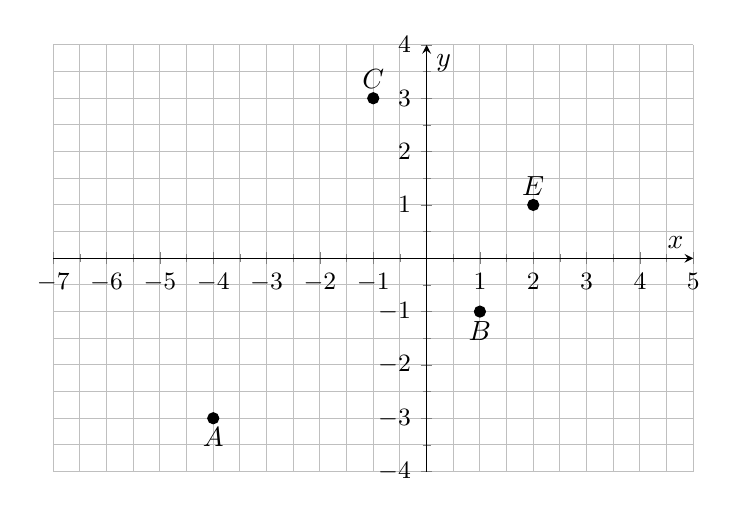
\begin{tikzpicture}\begin{axis}[coursaxe,axis equal image,xmin=-7,xmax=5,ymin=-4,ymax=4,width=12cm,height=7cm,xtick={-7,...,5},ytick={-4,...,4}]
\addplot[only marks]coordinates{(-4,-3)(1,-1)(-1,3)(2,1)};
\node[below]at(axis cs:-4,-3){$A$};\node[below]at(axis cs:1,-1){$B$};\node[above]at(axis cs:-1,3){$C$};\node[above]at(axis cs:2,1){$E$};
\ifprof\addplot[thick]coordinates{(-4,-3)(1,-1)(-1,3)(-6,1)(-4,-3)};\addplot[dashed,domain=-6:5]{.4*x-1.4};\addplot[dashed,domain=-2:5]{-2*x/3+7/3};\addplot[only marks]coordinates{(3.5,0)(0,-.333333)};\node[above]at(axis cs:-6,1){$D$};\node[above]at(axis cs:3.5,0){$K$};\node[below right]at(axis cs:0,-.33333){$F$};\fi
\end{axis}\end{tikzpicture}\end{center}
\reponse[4]{1. $D=A+C-B=(-6;1)$. 2. Midpoint of $[AC]$ and of $[BD]$: $I(-5/2;0)$. 3. $(AB):2x-5y-7=0$; $(CE):2x+3y-7=0$. Subtracting gives $8y=0$, then $x=7/2$, so $K(7/2;0)$. 4. $\vect{AE}=(6;4)$, so $F=A+(4;8/3)=(0;-1/3)$. $\vect{DF}=(6;-4/3)$, $\vect{DB}=(7;-2)$; determinant $-12+28/3=-8/3\ne0$. The three points are not collinear.}

\fiche{Comparing a vector method and a coordinate method}
\ex{In a non-degenerate triangle $ABC$, $I$ is the midpoint of $[AB]$ and $J$ the midpoint of $[AC]$.
\begin{enumerate}\item Prove with vectors that $(IJ)\parallel(BC)$.\item Check with $A(0;0)$, $B(6;0)$, $C(2;4)$.\item For these coordinates, determine the equations of $(IJ)$ and $(BC)$, then the ratio $IJ/BC$.\end{enumerate}}
\reponse[7]{1. $\vect{IJ}=\vect{IA}+\vect{AJ}=\frac12(\vect{BA}+\vect{AC})=\frac12\vect{BC}$. The vectors are nonzero and collinear.\\2. $I(3;0)$, $J(1;2)$; $\vect{IJ}=(-2;2)$ and $\vect{BC}=(-4;4)$.\\3. $(IJ):x+y-3=0$; $(BC):x+y-6=0$. Their direction vectors are collinear. $IJ=\sqrt8$, $BC=\sqrt{32}$, so $IJ/BC=1/2$. The vector proof is general; the numerical check only proves this particular case.}
\ex{A figure seems to show two parallel lines. What is the difference between this observation and a proof?}
\reponse[3.2]{The figure suggests a conjecture and may be imprecise. A proof uses exact data and a property, for example a zero determinant of nonzero direction vectors. A conclusion must state the objects concerned.}

\fiche{Recognising a configuration and justifying}
\ex[Original situation]{In an orthonormal frame, $A(0;0)$, $B(4;2)$, $C(3;4)$ and $D(-1;2)$.
\begin{enumerate}\item Show that $ABCD$ is a parallelogram.\item Calculate the four lengths and determine whether it is a rhombus.\item Calculate $AC^2$, $BD^2$ and determine whether it is a rectangle.\item Determine its centre and an equation of each diagonal.\end{enumerate}}
\reponse[8]{1. $\vect{AB}=(4;2)=\vect{DC}$: it is a parallelogram. 2. $AB=CD=\sqrt{20}=2\sqrt5$, $BC=DA=\sqrt5$; adjacent sides are not equal, so it is not a rhombus. 3. $AC^2=3^2+4^2=25$; $BD^2=(-5)^2+0^2=25$. A parallelogram whose diagonals have the same length is a rectangle. One can also use $AB^2+BC^2=20+5=25=AC^2$ and the converse of Pythagoras. 4. The centre is $I(3/2;2)$. $(AC):4x-3y=0$; $(BD):y=2$. Their intersection recovers $I$.}
\prof{Comparison of approaches: a proof by Pythagoras or by the property of the diagonals is enough. Do not impose the dot product, which is not needed here. For the oral part, distribute the methods among groups, then ask for a joint justification.}

\sequence{Synthesis problems, reasoning and fluency}{Synthesis and reasoning}{30 March--9 April 2027}
\section{Implication, converse and counterexample}
\begin{cours}[Tools to use in context]
``If $P$, then $Q$'' is an implication $P\Rightarrow Q$. Its converse is $Q\Rightarrow P$; it is not automatically true. An equivalence $P\iff Q$ requires both implications.
A counterexample is enough to refute a universal statement; a few examples are not enough to prove it. The contrapositive $\text{not }Q\Rightarrow\text{not }P$ is equivalent to $P\Rightarrow Q$.
\end{cours}
\ex{For an integer $n$: ``If $n$ is a multiple of $4$, then $n$ is even.'' Prove the implication, write its converse and its contrapositive, then say which are true.}
\reponse[5]{If $n=4k$, then $n=2(2k)$ is even. Converse: ``If $n$ is even, then $n$ is a multiple of $4$''; it is false with $n=2$. Contrapositive: ``If $n$ is odd, then $n$ is not a multiple of $4$''; it is true and equivalent to the original implication.}
\ex{For $x\in\R$, study ``$x=3\Rightarrow x^2=9$'' and its converse. Give a correct equivalence.}
\reponse[3.2]{The implication is true. The converse is false with $x=-3$. The correct equivalence is $x^2=9\iff x=3\text{ or }x=-3$. With the extra hypothesis $x\geq0$, one can write $x^2=9\iff x=3$.}
\prof{These notions are made explicit from the problems; they are not a standalone chapter of formal logic to memorise without context.}

\fiche{Negation, case analysis and proof}
\ex{Negate correctly: ``$x>2$''; ``$x\in[1;4]$''; ``All students play sport''; ``$A$ and $B$ both occur''.}
\reponse[4]{``$x\leq2$''; ``$x<1$ or $x>4$''; ``At least one student does not play sport''; ``$A$ does not occur or $B$ does not occur''. The ``or'' is inclusive.}
\ex{Show by case analysis that $n(n+1)$ is even for every integer $n$. Then show that $n^2+n+1$ is odd.}
\reponse[4]{If $n$ is even, $n(n+1)$ has an even factor. If $n$ is odd, $n+1$ is even; the product is again even. The two cases cover all integers. Since $n^2+n+1=n(n+1)+1$, it is an odd integer.}
\ex{A student writes ``$n^2$ even implies $n$ even, because I checked it for $n=2,4,6$''. Replace this justification with a proof.}
\reponse[3.2]{If $n$ were odd, the result proved in sequence 1 would give $n^2$ odd, a contradiction. This is a contrapositive argument, or presented here as a proof by contradiction. Three examples do not cover all integers.}

\fiche{Combining algebra, functions and percentages}
\ex[Original situation]{Two fictional rental rates are offered for $x$ hours, with $x\in[0;8]$: $A(x)=3000+2000x$ Ar and $B(x)=3500x$ Ar.
\begin{enumerate}\item Calculate the costs for $1$ h and $4$ h.\item Find where the rates are equal, then the durations for which $A$ is cheaper.\item A $10\,\%$ discount is granted on the whole of rate $A$. Give the new rate $A_r$ and the new comparison threshold.\end{enumerate}}
\reponse[6]{1. At $1$ h: $5000$ Ar versus $3500$ Ar. At $4$ h: $11000$ Ar versus $14000$ Ar. 2. $3000+2000x=3500x\iff x=2$. $A<B$ for $x>2$, so on $]2;8]$. 3. $A_r(x)=0.9(3000+2000x)=2700+1800x$. Equality with $B$ gives $1700x=2700$, that is $x=27/17\approx1.59$ h. $A_r<B$ on $]27/17;8]$. The discount also applies to the fixed charge.}
\begin{lstlisting}
def tarif_moins_cher(x):
    a = 3000 + 2000*x
    b = 3500*x
    if a < b:
        return "A"
    elif b < a:
        return "B"
    else:
        return "egalite"
\end{lstlisting}
\ex{Predict the results for $x=1,2,4$. Modify the line that computes $a$ to take the discount into account.}
\reponse[2.4]{Results: \texttt{"B"}, \texttt{"egalite"}, \texttt{"A"}. Replace with \texttt{a = 0.9*(3000 + 2000*x)}. The domain $[0;8]$ is assumed to be respected in the calls.}

\sequence{Probability: conditioning and weighted trees}{Probability}{26 April--24 May 2027}
\section{Sample space, outcomes and events}
\begin{cours}[Vocabulary]
A random experiment has several possible results, without it being known in advance which will occur. An outcome is a possible result; the sample space $\Omega$ is the set of them. An event is a subset of $\Omega$; an elementary event contains a single outcome.
The impossible event is $\varnothing$; the certain event is $\Omega$.
\end{cours}
\begin{cours}[Operations on events]
$\overline A$ is the complementary event of $A$. $A\cap B$ means ``$A$ and $B$''; $A\cup B$, ``$A$ or $B$'', possibly both. Two events are mutually exclusive if $A\cap B=\varnothing$; otherwise, they are compatible.
\end{cours}
\ex{A six-sided die is rolled. Write $\Omega$, $A$: ``get an even number'', $B$: ``get $4$'', then $\overline A$, $A\cap B$ and $A\cup B$. Are $A,B$ compatible?}
\reponse[4]{$\Omega=\{1;2;3;4;5;6\}$, $A=\{2;4;6\}$, $B=\{4\}$, $\overline A=\{1;3;5\}$, $A\cap B=\{4\}$, $A\cup B=A$. The events are compatible because they share the outcome $4$.}
\ex{With $A=\{a;b;c;d;e\}$ and $B=\{b;e;f;g;h\}$, give the intersection and the union. Can $\overline A$ be determined without specifying the sample space?}
\reponse[3.2]{$A\cap B=\{b;e\}$ and $A\cup B=\{a;b;c;d;e;f;g;h\}$. The complement depends on the sample space; it cannot be determined without this information.}

\fiche{Probability model and equally likely outcomes}
\begin{cours}[Probability on a finite sample space]
To each outcome, a model assigns a probability that is positive or zero; the sum is $1$. The probability of an event is the sum of the probabilities of its outcomes. We have
\[P(\Omega)=1,\quad P(\varnothing)=0,\quad P(\overline A)=1-P(A).\]
With equally likely outcomes, all outcomes have the same probability and
\[P(A)=\frac{\Card(A)}{\Card(\Omega)}.\]
Equal likelihood is an assumption of the model, not a consequence of the list of outcomes alone.
\end{cours}
\ex{Assume the die is fair. For $A=$ ``even'' and $C=$ ``greater than or equal to $5$'', calculate $P(A)$, $P(C)$, $P(A\cap C)$ and $P(A\cup C)$.}
\reponse[4]{$P(A)=3/6=1/2$, $P(C)=2/6=1/3$, $A\cap C=\{6\}$ so $P(A\cap C)=1/6$. $A\cup C=\{2;4;5;6\}$, so $P(A\cup C)=4/6=2/3$. The outcome $6$ must not be counted twice.}
\ex{A drawing pin can land point up or point down. Can we deduce that each outcome has probability $1/2$? How can a model be proposed?}
\reponse[4]{No: two outcomes are not enough to impose equal likelihood. One can repeat the throws under comparable conditions and use the observed frequencies to propose a model, bearing in mind fluctuations and the characteristics of the object.}
\prof{Reactivate the link between observed frequency and postulated probability. An experimental result does not prove exact equal likelihood.}

\fiche{Conditional probability from a table}
\begin{cours}[Definition]
For $P(A)>0$, the probability of $B$ given $A$ is
\[P_A(B)=\frac{P(A\cap B)}{P(A)},\qquad P(A\cap B)=P(A)P_A(B).\]
For an equally likely draw within a finite population:
\[P_A(B)=\frac{\Card(A\cap B)}{\Card(A)}.\]
We also write $P(B\mid A)$. $P_A(B)$ and $P_B(A)$ are generally not equal.
\end{cours}
\ex{A student is drawn uniformly from the class of $32$ students studied earlier. $G$: ``boy'', $N$: ``takes CS''.}
\begin{center}\renewcommand{\arraystretch}{1.5}\begin{tabular}{c|rr|r}
&$G$&$\overline G$&Total\\\hline
$N$&12&9&21\\$\overline N$&6&5&11\\\hline Total&18&14&32
\end{tabular}\end{center}
Calculate $P(G)$, $P(N)$, $P(G\cap N)$, $P_N(G)$ and $P_G(N)$.
\reponse[5]{$P(G)=18/32=9/16$, $P(N)=21/32$, $P(G\cap N)=12/32=3/8$.
$P_N(G)=12/21=4/7$, whereas $P_G(N)=12/18=2/3$.
By the formula: $P_N(G)=(12/32)/(21/32)=12/21$. Given that the student takes CS, the reference population is reduced to the $21$ students concerned.}
\vigilance{Conditioning requires the known event to have nonzero probability; we do not divide by zero.}

\fiche{Weighted trees and the probability of a path}
\begin{cours}[Rules]
At each node, the sum of the probabilities of the outgoing branches is $1$. A second-level branch carries a conditional probability. A path represents an intersection of events; its probability is the product of the probabilities written along that path.
\end{cours}
\begin{center}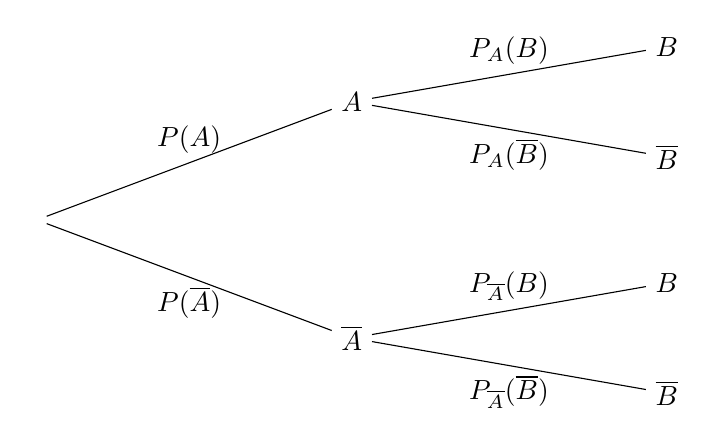
\begin{tikzpicture}[grow=right,level 1/.style={level distance=4cm,sibling distance=3cm},level 2/.style={level distance=4cm,sibling distance=1.4cm},edge from parent/.style={draw},every node/.style={font=\normalsize}]
\node{} child{node{$\overline A$} child{node{$\overline B$} edge from parent node[below]{$P_{\overline A}(\overline B)$}} child{node{$B$} edge from parent node[above]{$P_{\overline A}(B)$}} edge from parent node[below]{$P(\overline A)$}} child{node{$A$} child{node{$\overline B$} edge from parent node[below]{$P_A(\overline B)$}} child{node{$B$} edge from parent node[above]{$P_A(B)$}} edge from parent node[above]{$P(A)$}};
\end{tikzpicture}\end{center}
\ex{We know $P(A)=0.6$, $P_A(B)=0.7$ and $P_{\overline A}(\overline B)=0.9$. Complete the other branches and calculate the probabilities of the four paths.}
\reponse[5]{$P(\overline A)=0.4$, $P_A(\overline B)=0.3$, $P_{\overline A}(B)=0.1$.
\[P(A\cap B)=0.6\times0.7=0.42,\quad P(A\cap\overline B)=0.18,\]
\[P(\overline A\cap B)=0.04,\qquad P(\overline A\cap\overline B)=0.36.\]
The sum of the four probabilities is $1$, which checks the consistency of the model.}
\ex{Justify the multiplication along the path $A$ then $B$ from the definition of $P_A(B)$.}
\reponse[2.4]{Since $P_A(B)=P(A\cap B)/P(A)$ and $P(A)>0$, multiplying by $P(A)$ gives $P(A)P_A(B)=P(A\cap B)$.}

\fiche{From a table to a tree}
\ex{For the class of $32$ students, construct a tree starting with CS / no CS, then boy / girl. Then construct the tree in the reverse order. Check, in both trees, the probability of choosing a girl who takes CS.}
\reponse[7]{First tree: initial branches $P(N)=21/32$, $P(\overline N)=11/32$. After $N$: $P_N(G)=12/21=4/7$, $P_N(\overline G)=9/21=3/7$. After $\overline N$: $6/11$ and $5/11$.
Second tree: initial branches $P(G)=18/32=9/16$, $P(\overline G)=14/32=7/16$. After $G$: $P_G(N)=12/18=2/3$, then $1/3$. After $\overline G$: $P_{\overline G}(N)=9/14$, then $5/14$.
The required path is worth $(21/32)(9/21)=9/32$ in the first tree and $(14/32)(9/14)=9/32$ in the second. Changing the order preserves the probabilities of the intersections but changes the probabilities of the branches.}
\ex{An urn contains $3$ red balls and $2$ blue balls. Two balls are drawn in succession \textbf{without replacement}. Construct the tree of colours and calculate the probability of drawing two red balls.}
\reponse[5]{First level: $R$ with $3/5$, $B$ with $2/5$. After $R$, $2$ red and $2$ blue remain: branches $1/2,1/2$. After $B$, $3$ red and $1$ blue remain: branches $3/4,1/4$. So $P(R_1\cap R_2)=(3/5)(1/2)=3/10$. Using $3/5$ on the second red branch would ignore the absence of replacement.}

\fiche{Inverting conditioning and false positives}
\ex[Fictional component check]{A batch contains $10000$ components, of which $100$ are defective. A test is positive for $99$ of the defective components and for $495$ of the non-defective components. A component is chosen uniformly. $D$: ``defective''; $T$: ``test positive''.
\begin{enumerate}\item Complete the two-way table of test / true state.\item Calculate $P_D(T)$ and $P_T(D)$.\item Give the number of false positives and false negatives.\item Calculate the sensitivity $P_D(T)$ and the specificity $P_{\overline D}(\overline T)$.\end{enumerate}}
\reponse[7]{
\begin{center}\renewcommand{\arraystretch}{1.5}\begin{tabular}{c|rr|r}&$D$&$\overline D$&Total\\\hline $T$&99&495&594\\$\overline T$&1&9405&9406\\\hline Total&100&9900&10000\end{tabular}\end{center}
$P_D(T)=99/100=99\,\%$. On the other hand $P_T(D)=99/594=1/6\approx16.67\,\%$. A positive test therefore does not imply here a $99\,\%$ probability of defect.
The $495$ false positives are the sound components that tested positive; the false negative is the defective component that tested negative. The sensitivity is $99\,\%$; the specificity $9405/9900=95\,\%$.
The low initial proportion of defective components explains why false positives outnumber true positives despite the good sensitivity.}
\begin{cours}[Reading a test result]
``Positive among the defective'' and ``defective among the positives'' correspond to two different conditionings. Always name the reference group before the calculation.
\end{cours}
\prof{The numbers are fictional. The table allows studying the inversion without requiring a general total-probability formula: this is not an expectation of the 2026 Seconde programme.}

\fiche{Simulation and the law of large numbers}
\begin{cours}[Popularised version]
When an experiment is repeated a large number of times in the same model with independent repetitions, the observed frequency of an event is, barring exceptions, close to its probability. It fluctuates: it does not necessarily get closer with each new trial.
\end{cours}
\begin{lstlisting}
from random import Random

def frequences_six(n, graine=1):
    # n entier >= 1 ; modele de lancers independants
    rng = Random(graine)
    succes = 0
    frequences = []
    for k in range(1, n+1):
        if rng.randint(1, 6) == 6:
            succes = succes+1
        frequences.append(succes/k)
    return frequences
\end{lstlisting}
\ex{Plot the frequencies for $n=1000$, with several seeds. Compare with $1/6$. Why fix the seed? Can we require the final frequency to be exactly $1/6$?}
\reponse[4]{The plots depend on the seed and fluctuate around $1/6$. Fixing the seed makes the simulation reproducible. With $1000$ throws, a final frequency of exactly $1/6$ is even impossible, because $1000/6$ is not an integer. A nearby frequency is consistent with the model, but is not a proof of it.}
\ex{Modify the program to track the frequency of the event ``even result''. Which reference probability should be used?}
\reponse[3.2]{Replace the test with \texttt{rng.randint(1, 6) \% 2 == 0}. The reference probability is $3/6=1/2$. Each trial must make a single draw; do not call the generator several times to test the same result.}

\sequence{Consolidation and transition to Year 12}{Annual review}{25 May--11 June 2027}
\section{Review of calculation, functions and geometry}
\ex[Annual review -- part A]{\begin{enumerate}
\item Reduce $168/252$ to lowest terms; calculate $2^{-3}+1/4$.
\item Factorise $x^2-6x+9$, then solve $(x-3)^2=4$.
\item Solve $\dfrac{x-2}{x+1}\geq0$.
\item For $f(x)=4-(x-1)^2$ on $[-2;3]$, give the maximum and the abscissae where $f(x)=0$.
\item With $A(0;1)$, $B(4;3)$, $C(6;4)$, prove collinearity and give an equation of the line.
\end{enumerate}}
\reponse[9]{1. $168/252=2/3$, and $2^{-3}+1/4=1/8+2/8=3/8$. 2. $(x-3)^2$; $x-3=\pm2$, so $S=\{1;5\}$. 3. Forbidden $-1$, zero $2$; signs $+,-,+$, so $S=]-\infty;-1[\cup[2;+\infty[$. 4. The square is positive or zero, so $f(x)\leq4$, with equality at $x=1$. The zeros are $x=-1,3$, both in the domain. 5. $\vect{AB}=(4;2)$, $\vect{AC}=(6;3)=\frac32\vect{AB}$. An equation is $x-2y+2=0$.}
\prof{Indicative marking: 10 points, 2 per question. For question 3, reserve one point for the domain and the endpoints. For question 5, ask for the conclusion after the calculation.}

\fiche{Review of data, probability and modelling}
\ex[Annual review -- part B]{\begin{enumerate}
\item Calculate the mean and median of $2;4;4;6;9$. Determine $Q_1,Q_3$.
\item A price drops by $15\,\%$, then rises by $20\,\%$. Give the overall rate and the rate that then restores the initial price.
\item In a fictional population of $100$ people, $40$ play sport ($S$), $30$ come by bike ($V$), $18$ do both. Construct the two-way table and calculate $P_S(V)$, $P_V(S)$ for an equally likely draw.
\item For a rectangle of perimeter $24$ m, express the area as a function of one dimension $x$ and prove its maximum.
\end{enumerate}}
\reponse[9]{1. Mean $25/5=5$, median $4$. Quartile ranks $2$ and $4$, so $Q_1=4$, $Q_3=6$.\\2. Overall multiplier $0.85\times1.20=1.02$: an increase of $2\,\%$. Reverse rate $1/1.02-1=-1/51\approx-1.96\,\%$.\\3. Table: $S\cap V=18$, $S\cap\overline V=22$, $\overline S\cap V=12$, $\overline S\cap\overline V=48$. $P_S(V)=18/40=45\,\%$, $P_V(S)=18/30=60\,\%$.\\4. $A(x)=x(12-x)=36-(x-6)^2$ on $]0;12[$. The maximum is $36$ m$^2$, attained for the square of side $6$ m.}
\prof{Indicative marking: 10 points, respectively 2, 2, 3, 3. The review of parts A and B can be offered in one hour, then revisited with the course materials.}

\fiche{Choosing a strategy and preparing what comes next}
\ex[A program to explain]{For a given function $f$, explain the following program. What does it return with $f(x)=x^2$?}
\begin{lstlisting}
def tableau(f):
    valeurs = []
    for x in range(-3, 4):
        valeurs.append((x, f(x)))
    return valeurs
\end{lstlisting}
\reponse[3.2]{It returns a list of abscissa--image pairs for the integers from $-3$ to $3$ inclusive: $(-3,9),(-2,4),(-1,1),(0,0),(1,1),(2,4),(3,9)$. The bound $4$ of \texttt{range} is excluded. The table does not describe the images of all real numbers between $-3$ and $3$.}
\begin{cours}[Six skills to mobilise]
\textbf{Search}: try things out, organise leads. \textbf{Model}: choose variables, domain and assumptions. \textbf{Represent}: move from text to table, figure or graph. \textbf{Reason}: justify and distinguish conjecture from proof. \textbf{Calculate}: choose a form and check the operations. \textbf{Communicate}: explain clearly with suitable notation and units.
\end{cours}
\ex[End-of-year portfolio]{Choose a successful piece of work and a corrected one. For each, identify the skills used, explain one method and state a personal goal for the following year. Then redo an exercise matching this goal without looking at the correction.}
\reponse[4]{There is no single numerical answer. A satisfactory piece of work precisely identifies the problem, the chosen method, a justification and a check. The goal must be observable, for example: ``state the forbidden values before solving a quotient equation'', rather than ``get better at calculation''.}
\prof{To present the Year 12 pathways, rely on the courses actually offered in the school and their programmes in force. The booklet sets no automatic mark threshold for guidance.}

\ifprof
\clearpage\renewcommand{\titreseq}{Teacher annexes}\addcontentsline{toc}{section}{Teacher annexes: use and correspondence}
\section*{Using the common source}
\begin{cours}[One source, two versions]
The line \texttt{\string\proffalse} in the preamble produces the student version; replacing it with \texttt{\string\proftrue} produces the teacher version. The statements and course content are common. Answers, written-out proofs, corrected figures and pedagogical cues appear only in teacher mode.
\end{cours}
All graphs and diagrams are written in TikZ/PGFPlots. No external image or page of the original PDF is needed for compilation. Compile twice with PDFLaTeX to update the table of contents and the links. The two PDFs may have different pagination; the stable references are the sequence and example numbers.
\begin{methode}[Implementation cues]
\begin{itemize}
\item Before an example: have students restate the data and the question; allow a preparatory representation.
\item During the investigation: provide targeted help (first step, diagram, simple case) and an extension for students who have finished.
\item During the correction: separate result, method, justification and verification. Have a frequent error explained.
\item For fluency work: mix recent and older questions, then redo the fragile ones after a delay.
\item For language: make explicit ``among'', ``at least'', ``if'', ``and'', ``or'' and the meaning of the symbols before calculating.
\end{itemize}
\end{methode}
\section*{Common criteria for a piece of work}
\begin{center}\small\renewcommand{\arraystretch}{1.6}\begin{tabularx}{\linewidth}{l X}
Search&An approach is under way; the attempts provide information.\\
Model&The variables, domain and assumptions match the situation.\\
Represent&The table, graph or diagram is readable, labelled and consistent.\\
Reason&Properties are applied under their conditions; the conclusion follows.\\
Calculate&The operations are correct; exact values are kept when necessary.\\
Communicate&The write-up answers the question, with appropriate units and precision.
\end{tabularx}\end{center}
For each criterion, four levels can be used: not started, partial, correct with help, independent. This grid is used to give usable feedback; it does not replace a marking scheme specific to an assessment.

\clearpage\section*{Correspondence with the original booklet}
\begin{center}\small\renewcommand{\arraystretch}{1.5}\begin{tabularx}{\linewidth}{p{6.3cm} X}
\textbf{Sequences of the supplied booklet}&\textbf{Destination in this adaptation}\\\hline
1. Algebraic calculation&8; reactivation in the starter routines from the start of the year.\\
2. Numbers and calculations&1 for arithmetic; 4 for sets; 8 for powers, fractions and roots.\\
3. Intervals and absolute value&4; reuse of the absolute value function in 6 and 10.\\
4. Equations and inequalities&8; simple equations reactivated in 3 and 6.\\
5. Proportion and percentage change&9.\\
6. Vectors&2.\\
7. Functions and graphical representation&6 for representations and readings; 10 for variations and extrema.\\
8. Notions of probability&14; set vocabulary introduced in 1.\\
9. Notions of collinearity&2; major synthesis moved to 12.\\
10. Sign tables and inequalities&8.\\
11. Statistics&7, with additions on graphs and the estimated median.\\
12. Lines and systems&3.\\
13. Reference functions (4 parts)&3 for the affine line; 6 for the reference functions and solving; 10 for variations.\\
14. Frequencies and conditional probabilities&11 for frequencies; 14 for conditioning and trees.\\\hline
Progression slots with no direct equivalent&5, 12, 13, 15: reviews, syntheses and consolidation created.
\end{tabularx}\end{center}
The layout is rebuilt in the spirit of the model: A4 portrait, serif typography, black boxes, gridded areas, examples and proofs. The recomposition and the change of order are not a page-by-page facsimile. Pagination is continuous; the contents page no longer uses page numbers that restart at each former sequence.
The usable numerical examples of the model have been kept. Ambiguous figures have been replaced by curves whose expression allows an exact check. The developments on square root, cube, simulation, cross-tabulated data and reviews complete the progression. Added situations with invented data are flagged as fictional; a class data collection is proposed so as to also work on real data.

\clearpage\section*{Substantive corrections made to the model}
\begin{enumerate}
\item \textbf{Powers.} The repeated product holds for a strictly positive integer exponent; negative exponents require a nonzero base.
\item \textbf{Fractions.} A zero quotient must be defined; only a nonzero fraction has an inverse. Simplifications do not remove the initial restrictions.
\item \textbf{GCD.} The two integers are not both zero in the definition by the greatest divisor; $\pgcd(0,0)=0$ is a separate convention.
\item \textbf{Vectors.} The zero vector directs no line. The characterisation $\vec u=k\vec v$ requires $\vec v\ne\vec0$, or a separate treatment of the zero case. Multiplication by any real number is made explicit.
\item \textbf{Equations of lines.} The condition is $(a,b)\ne(0,0)$; the order of the vectors in the determinant has been made consistent. $\vect{AM}$ can be zero when $M=A$ and is then not a direction vector.
\item \textbf{Intervals.} $0$ is excluded from the set of strictly negative real numbers. Infinities are not real numbers.
\item \textbf{Roots.} The positivity conditions and $\sqrt{x^2}=|x|$ are explicit. A formula that is false in general is not necessarily an inequality that is always true.
\item \textbf{Functions.} Images and preimages are distinguished; the domains of the curves cover the requested values. Graphical readings are not displayed with unjustified precision. The inverse function is not declared decreasing on the whole of $\R^*$.
\item \textbf{Statistics.} The median uses ``at least half''. Adding a value does not make the range decrease. The recalculations use the exact sum $1217$. Variance and standard deviation are not linear functions of the data: their correct transformations are specified.
\item \textbf{Classes.} A continuous data set is not defined by its grouping alone. The mean from the centres and the interpolated median are estimates under assumptions, distinct from the exact values.
\item \textbf{Interpretation.} Multiplying marks is not equated with raising difficulty. Proportion, rate and percentage points are distinguished.
\item \textbf{Probability.} Reference populations and model assumptions are named. Inversion of conditioning, false positives, false negatives and fluctuations are worked on. No general total-probability formula is required.
\item \textbf{Optimisation.} The sweep gives a maximum on a grid; a separate proof establishes the maximum on the interval. A bisection for finding a zero is not presented as a general optimisation method.
\end{enumerate}

\clearpage\section*{References and coverage check}
\textbf{Progression document used:} \emph{Programmation annuelle Seconde 2026--2027 rectifiée finale}, DOCX supplied. Dates and fifteen stages kept; the dates indicate ranges, not sessions on public holidays.
\par\textbf{Starting document:} \emph{Livret\_2nde\_\_\_Eleve.pdf}, 91 pages, supplied for this adaptation. The original LaTeX source was not attached, so the present source is a reconstruction.
\par\textbf{Official programme:} order of 26 February 2026, BO no.~14 of 2 April 2026, NOR MENE2602914A, applicable from the 2026--2027 school year:
\par\url{https://www.education.gouv.fr/bo/2026/Hebdo14/MENE2602914A}
\par\textbf{Resources supplied:} Seconde programme; resources ``Automatismes 2de'' and ``Raisonnement et démonstration 2de''. The booklet does not claim to reproduce these resources in full.
\begin{center}\small\renewcommand{\arraystretch}{1.5}\begin{tabularx}{\linewidth}{p{8cm} X}
\textbf{Area / skill}&\textbf{Sequences}\\\hline
Integers, multiples, parity, irreducible fractions&1, 5, 8, 13\\
Real numbers, intervals, distance, bounds&4, 5, 8\\
Algebra, powers, roots, equations and signs&8; starter routines all year\\
Vectors, bases, coordinates, norms, determinant&2, 12\\
Equations of lines and intersections&3, 12\\
Representations and six reference functions&6, 10\\
Variations, extrema, comparison, optimisation&10, 13, 15\\
Proportions and percentage change&9, 13, 15\\
Statistics, spread, classes, histogram, cumulative frequencies&7\\
Two-way tables, frequencies, real data&11\\
Conditioning, trees, inversion, simulation&14\\
Logic, proofs, Python, six skills&Spread across the sequences and reviews
\end{tabularx}\end{center}
\textbf{Mathematical check:} the numerical calculations, algebraic expressions, solution sets, table data, coordinates and programs were proofread and checked by calculation. For open collections and productions, the correction gives validity criteria rather than an invented result. Estimates and models remain explicitly flagged.
\fi

\end{document}
